\chapter{科研日志}
\section{2019.08.09}
今天的主要的主要工作是寻找一个合适的\TeX 模板,由于以前使用的latex模板在处理包含大量图片的文件时不仅非常慢,而且有许多图片存在显示不全的问题,所以准备了一个可以用pdflatex或xelatex编译的模板,但是目前这个模板也存在一些问题,正在修改,并且准备利用两天的时间将以前的笔记重新整理到这个模板下。另外,还给出了前几天完成的WS4模型给出的比结合能,已经对$V_{1p1n}$相互作用的描述。
\begin{figure}[H]
\centering
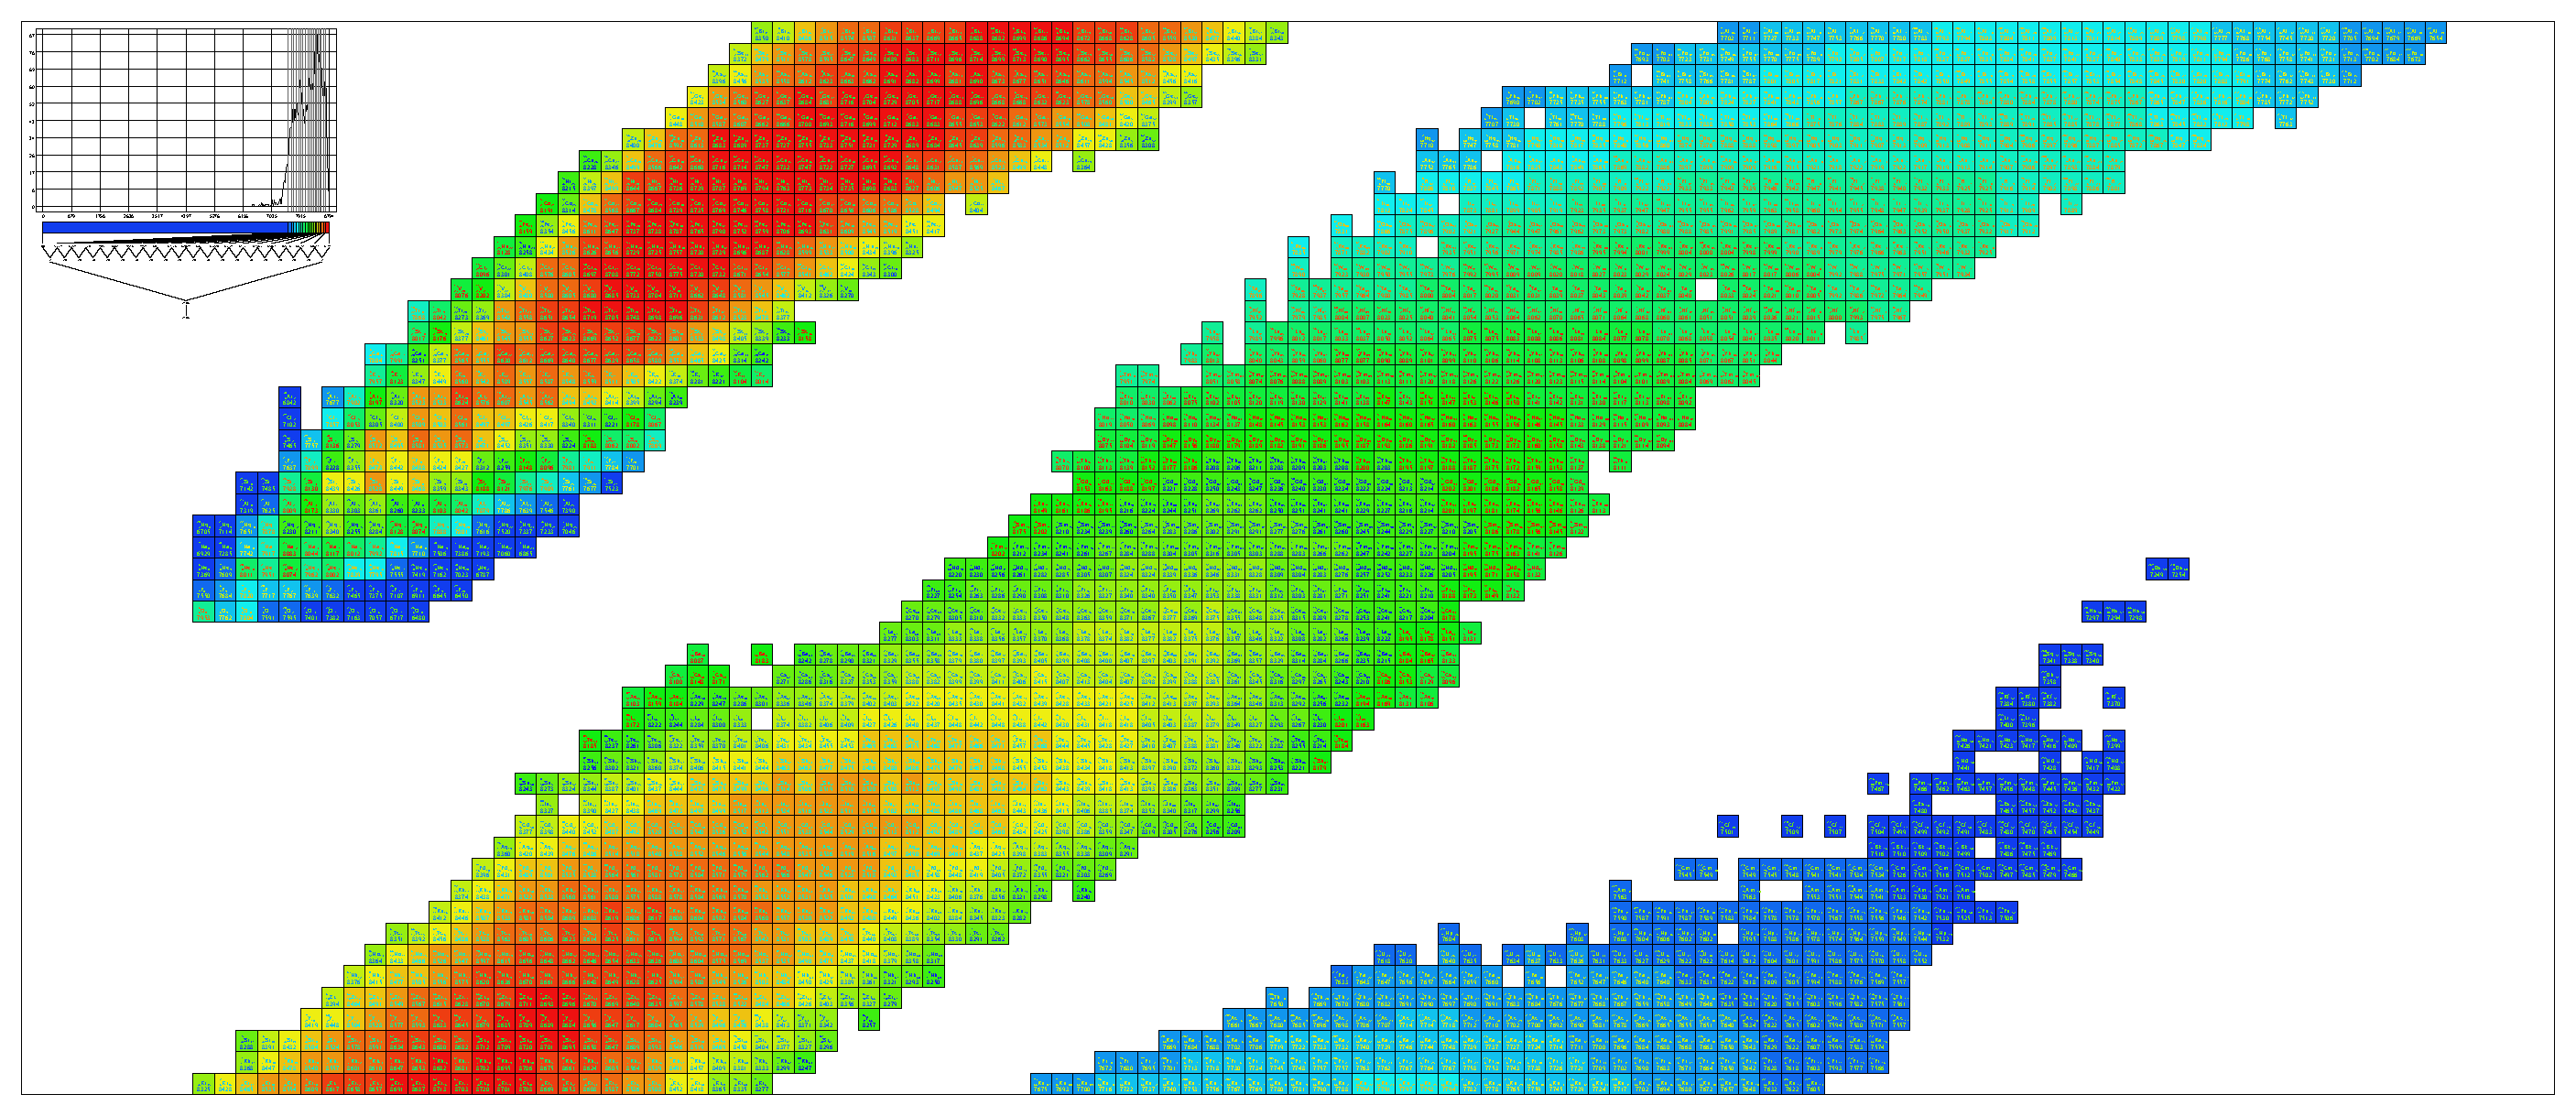
\includegraphics[width=0.9\textwidth]{figure/WS4perA.pdf}
\caption{WS4模型给出的比结合能在核素图中的分布.\label{fig_WS4perA}}
\end{figure}
\begin{figure}[H]
\centering
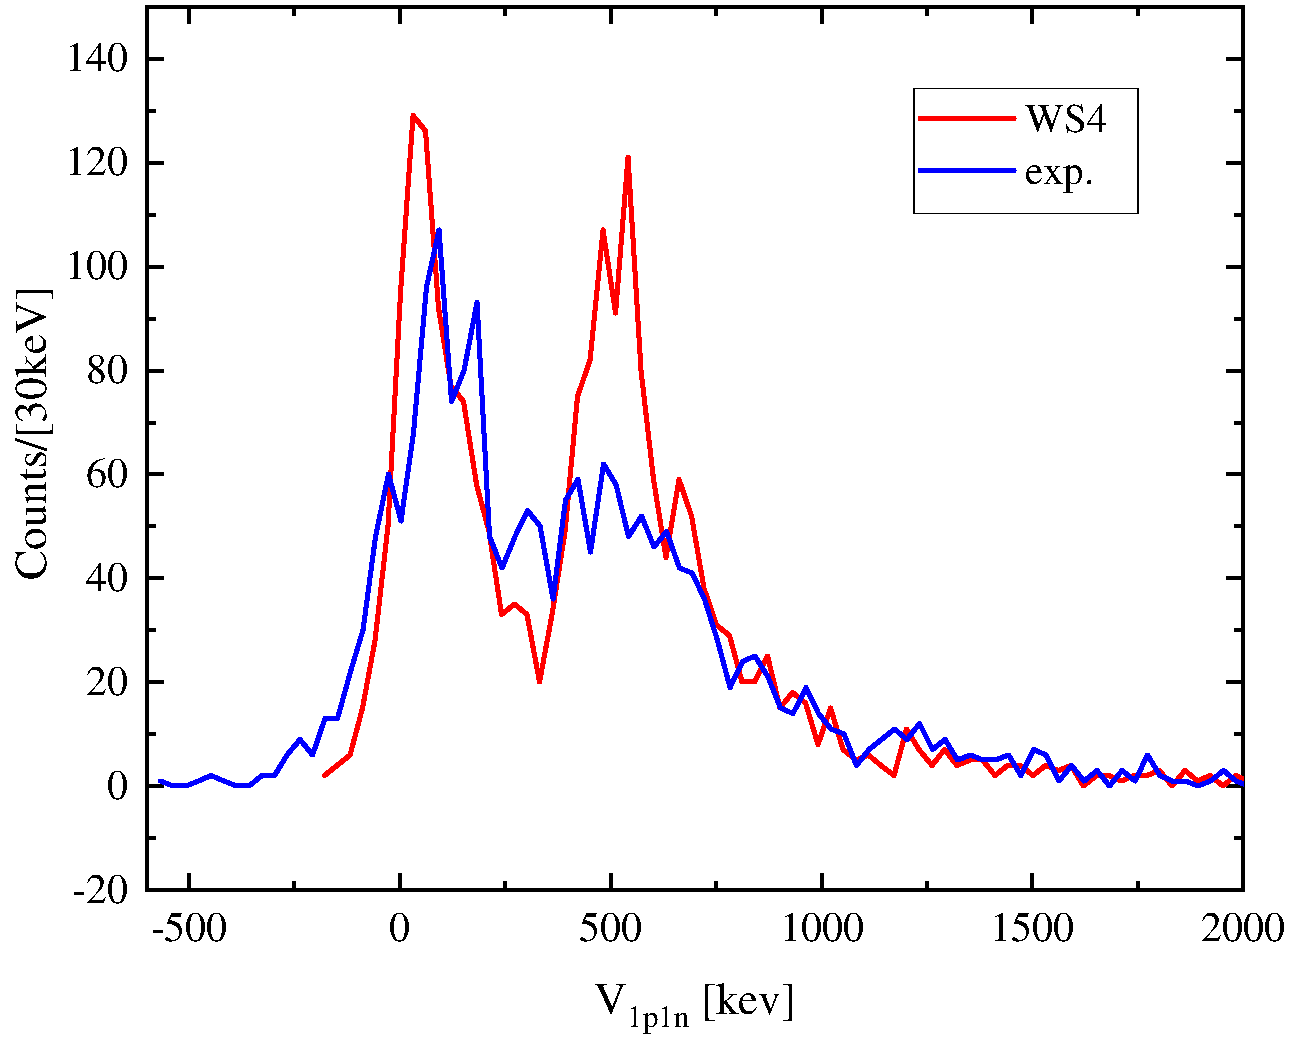
\includegraphics[width=0.6\textwidth]{figure/WS4V1p1n.pdf}
\caption{WS4模型给出的$V_{1p-1n}$相互作用的统计分布.\label{fig_WS4V1p1n}}
\end{figure}
\section{2019.08.18}
今天的工作主要是重新将基于质量表的核子相互作用部分整理为了 \TeX 的笔记,还有部分没有完成。
\section{2019.08.19}
今天的主要工作是对AME2016和FRDM模型的奇A核和偶A核的$V_{1p-1n}(Z,N)$相互作用的统计分布进行了高斯拟合见图\ref{fig_FRDMexpV1p1nt}和图\ref{fig_FRDMexpV1p1n}。
\begin{figure}[H]
\centering
\subfigure[对FRDM模型的奇A核和偶A核的$V_{1p-1n}(Z,N)$相互作用的统计分布进行的高斯拟合.\label{fig_FRDMV1p1n100}]{
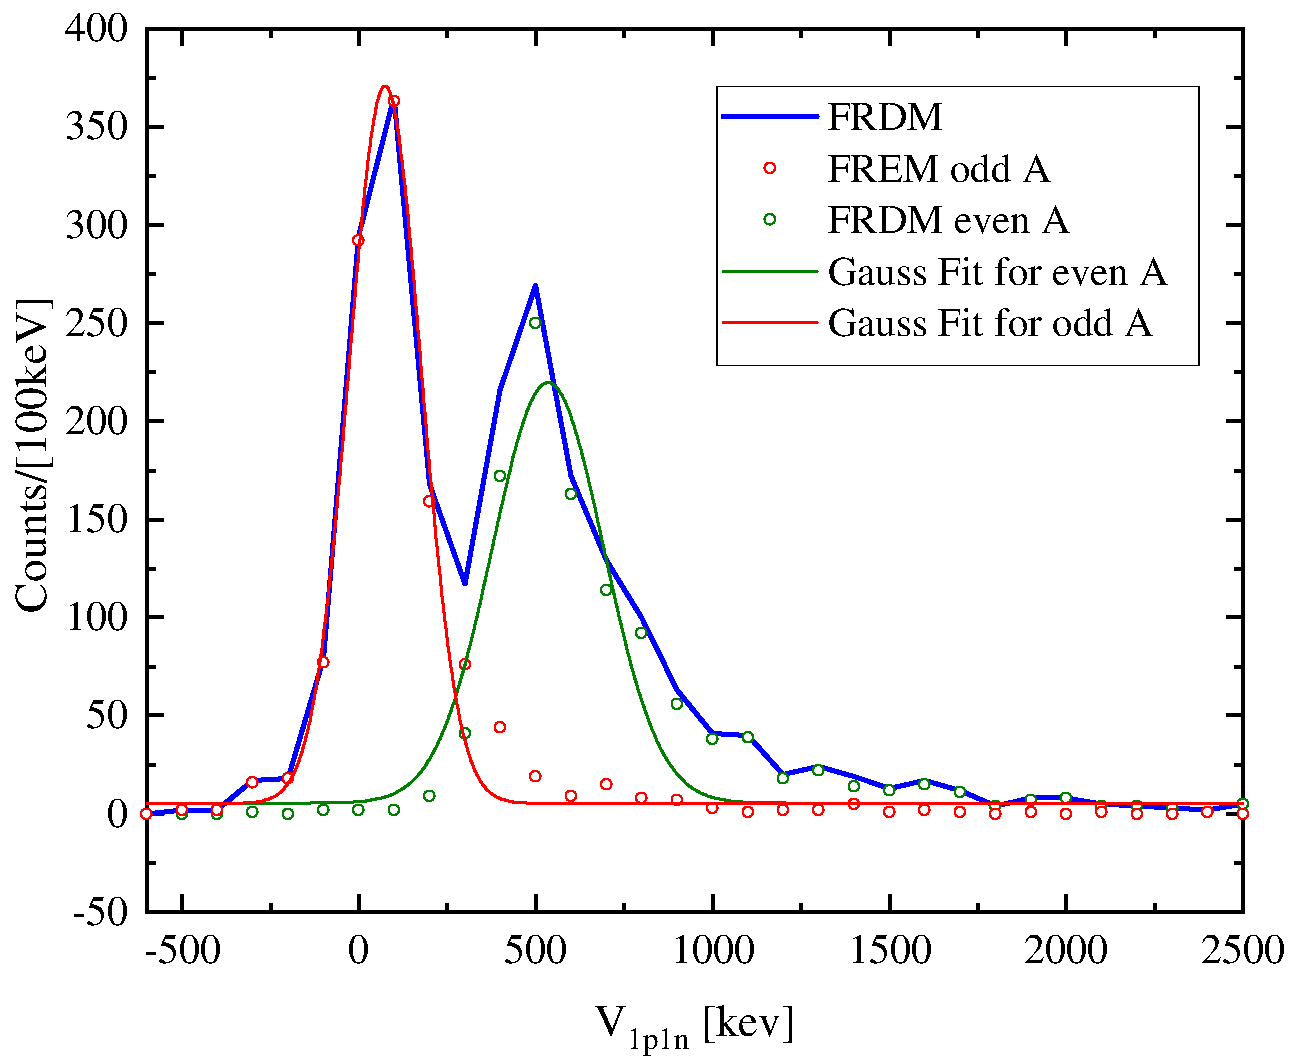
\includegraphics[width=0.4\textwidth]{figure/FRDMV1p1n100.pdf}}
\qquad
\subfigure[对AME2016的奇A核和偶A核的$V_{1p-1n}(Z,N)$相互作用的统计分布进行的高斯拟合.\label{fig_expV1p1n100}]{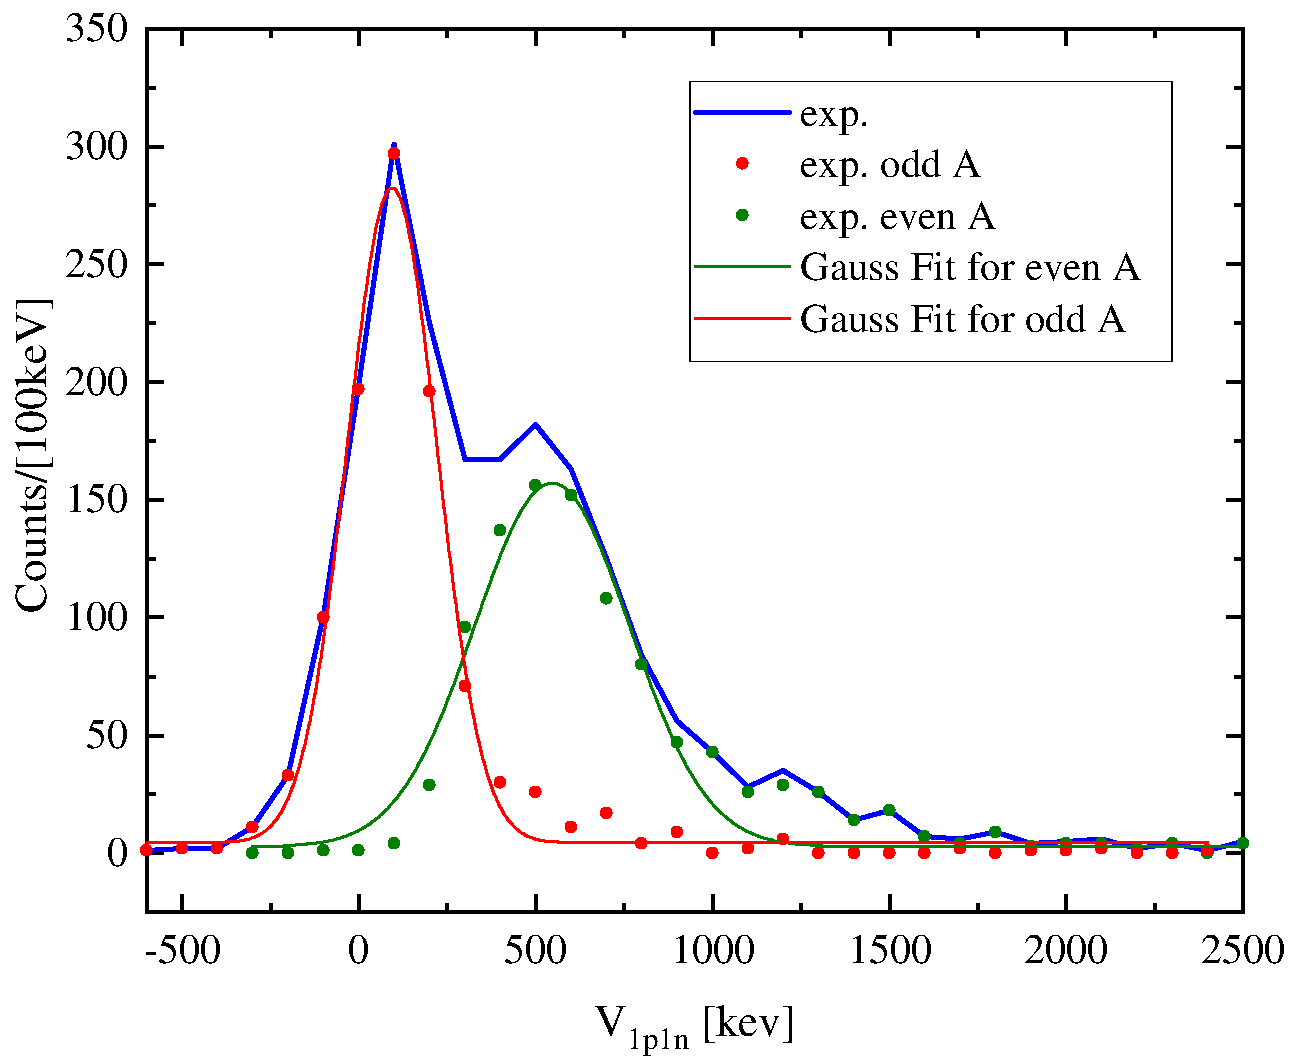
\includegraphics[width=0.4\textwidth]{figure/expV1p1n100.pdf}}
\caption{对AME2016和FRDM模型的奇A核和偶A核的$V_{1p-1n}(Z,N)$相互作用的统计分布进行的高斯拟合.\label{fig_FRDMexpV1p1nt}}
\end{figure}
\begin{figure}[H]
\centering
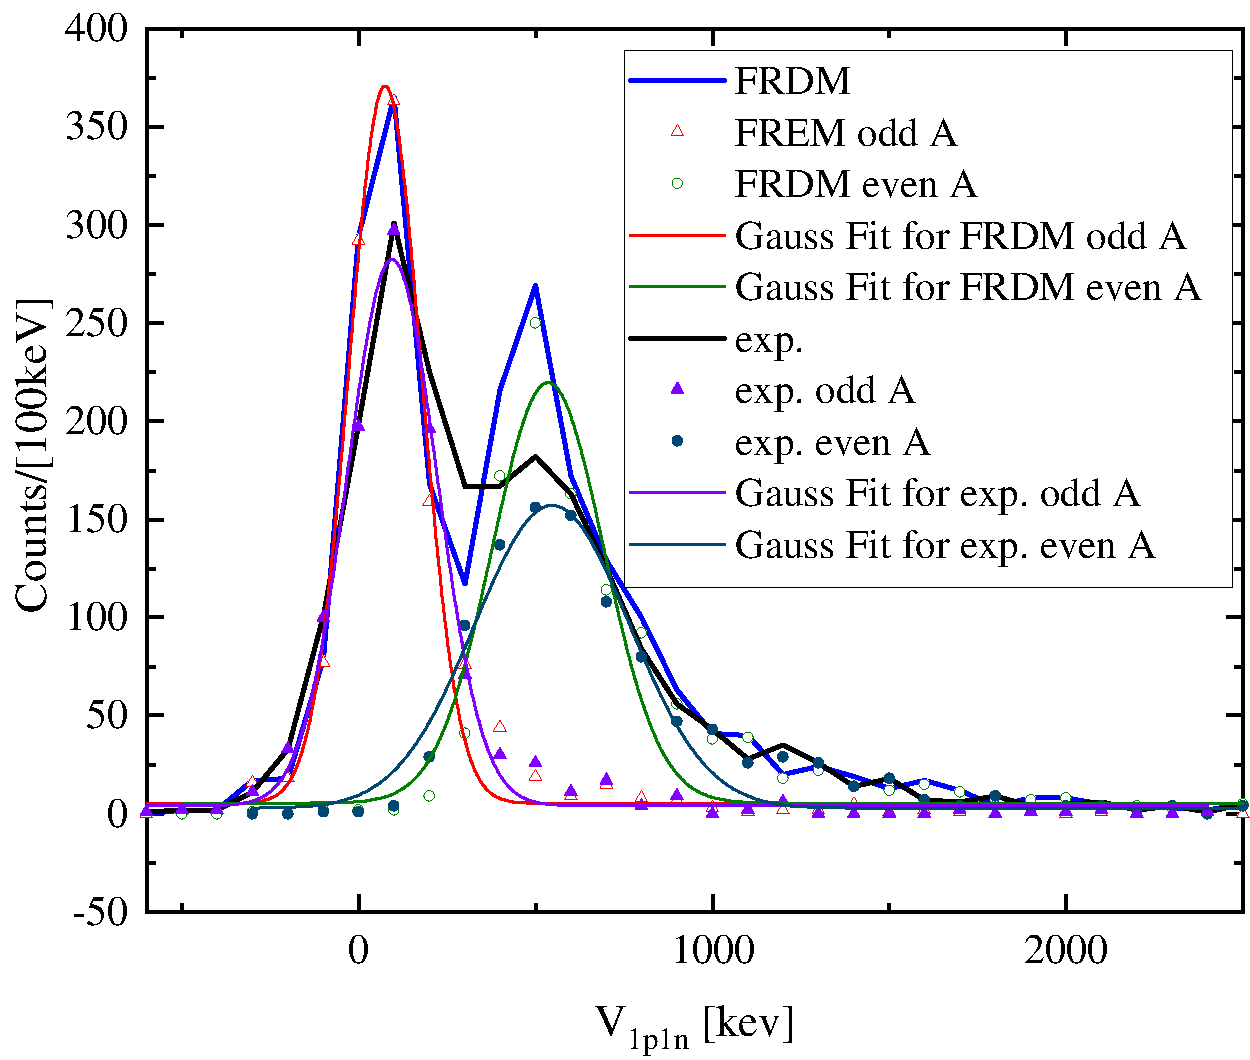
\includegraphics[width=0.5\textwidth]{figure/FRDMexpV1p1n.pdf}
\caption{分别对AME2016和FRDM模型的奇A核和偶A核的$V_{1p-1n}(Z,N)$相互作用的统计分布进行的高斯拟合.\label{fig_FRDMexpV1p1n}}
\end{figure}
\section{2019.08.21}
今天的主要工作是想要寻找一个合适的拟合公式来拟合$V_{1p-1n}(N,Z)$相互作用的统计分布,主要尝试了两类公式:
\begin{equation}
V=a(x-c)^2e^{-b(x-c)^2}\label{Yukawa}
\end{equation}
以及类似于 Planck 提出的黑体辐射公式:
\begin{equation}
	V=\frac{a}{(x-c)^5}\frac{1}{e^{\frac{b}{x-c}}-1} \label{Planck}
\end{equation}
其中$a,~b,~c$均为拟合参数,由于这两个函数都不能通过 origin 的最小二乘法拟合,所以利用 python 程序对公式\ref{Planck}进行了拟合,结果如图\ref{fig_Fit}
\begin{figure}[H]
\centering
\subfigure[利用公式\ref{Yukawa}对AME2016的偶A核的$V_{1p-1n}(Z,N)$相互作用进行的拟合.\label{fig_Yukawa}]{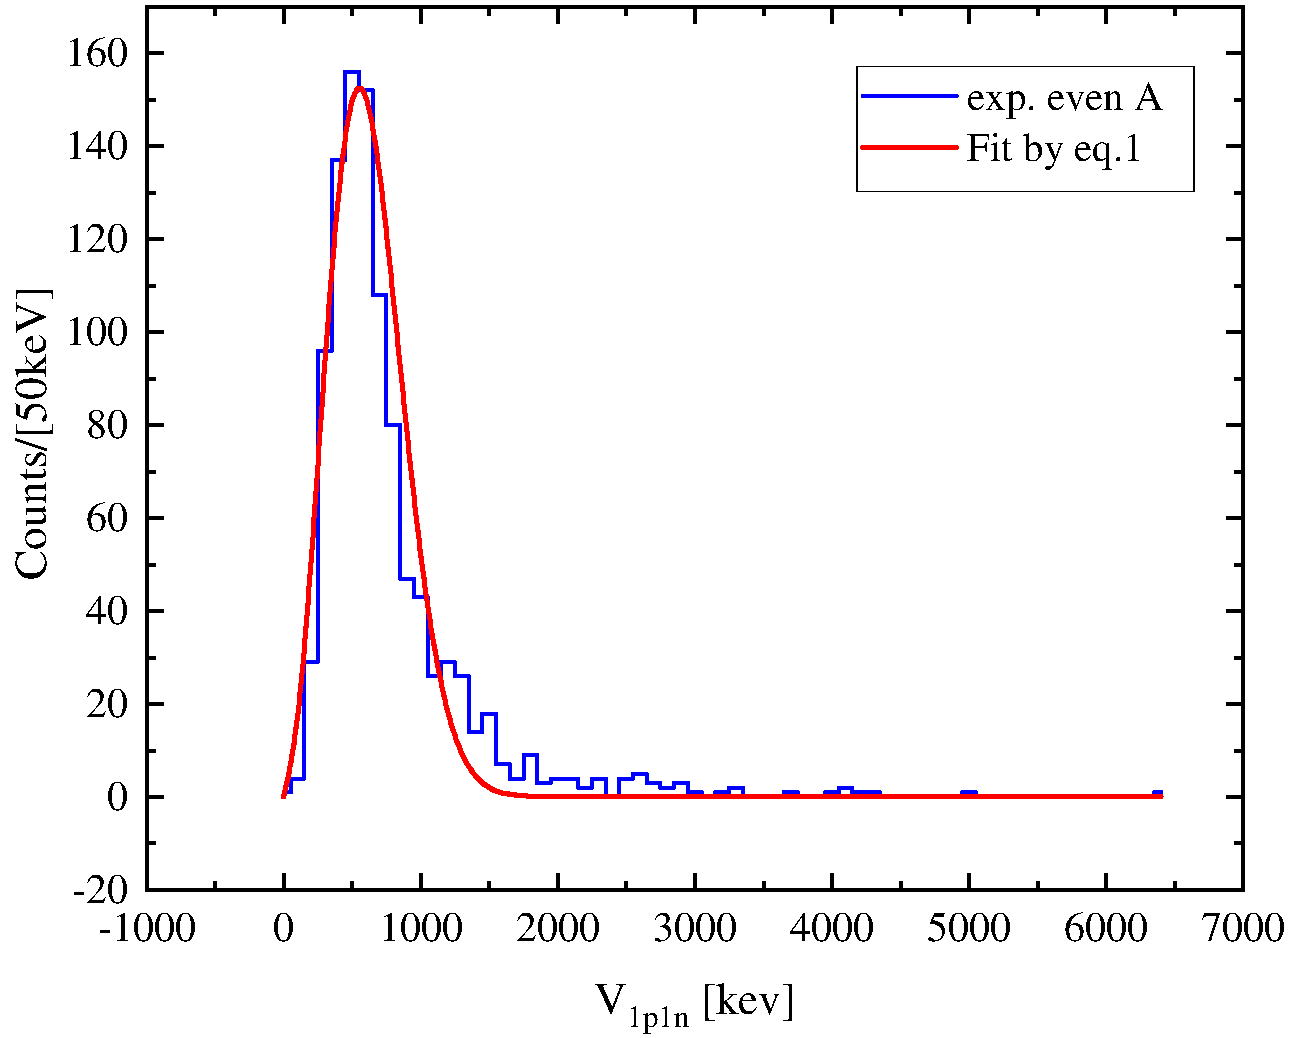
\includegraphics[width=0.4\textwidth]{figure/YFitexpV1p1neA.pdf}}
\qquad
\subfigure[利用公式\ref{Planck}对AME2016的偶A核的$V_{1p-1n}(Z,N)$相互作用进行的拟合.\label{fig_Planck}]{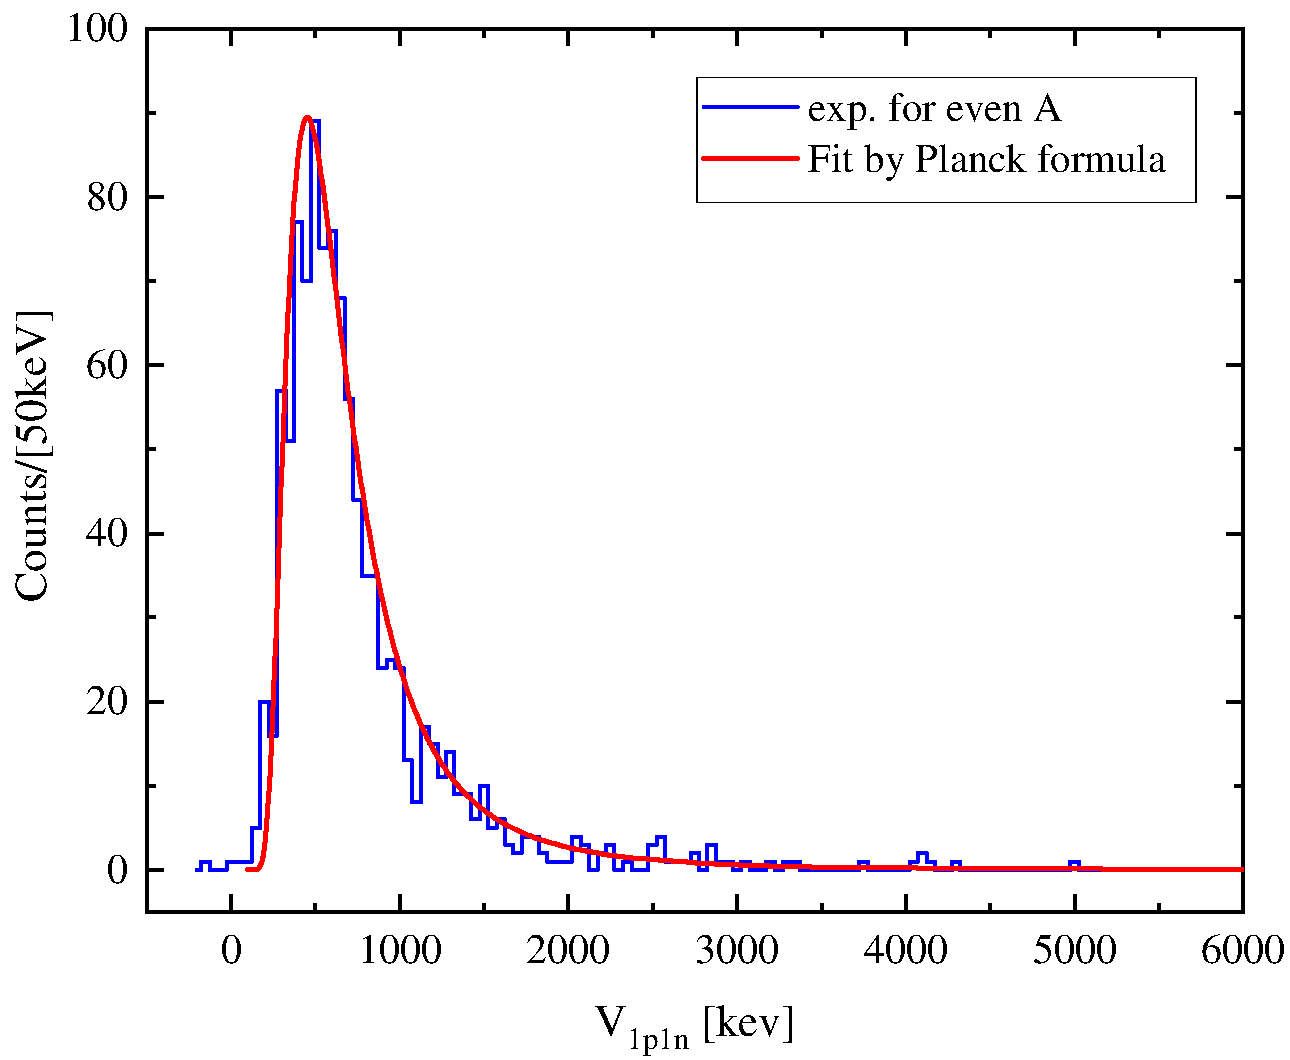
\includegraphics[width=0.4\textwidth]{figure/PFitexpV1p1neA.pdf}}
\caption{对AME2016偶A核的$V_{1p-1n}(Z,N)$相互作用的统计分布进行的拟合.\label{fig_Fit}}
\end{figure}
\section{2019.08.22}
今天的主要工作是发现Planck 提出的黑体辐射公式\ref{Planck}虽然可以比较好的描述AME2016的偶A核的$V_{1p-1n}(Z,N)$相互作用的统计分布,但是却不能很好的符合奇A核的$V_{1p-1n}(Z,N)$相互作用的统计分布,所以今天又在公式、\ref{Yukawa}的基础上做了改进:
\begin{equation}
V=a(x-c)^de^{-b(x-c)^e}\label{Yukawa2}
\end{equation}
其中$a,~b,~c,~d,~e$均为拟合参数,其拟合结果如图:
\begin{figure}[H]
\centering
\subfigure[利用公式\ref{Yukawa2}对AME2016的偶A核的$V_{1p-1n}(Z,N)$相互作用进行的拟合.\label{fig_Y3FiteA50}]{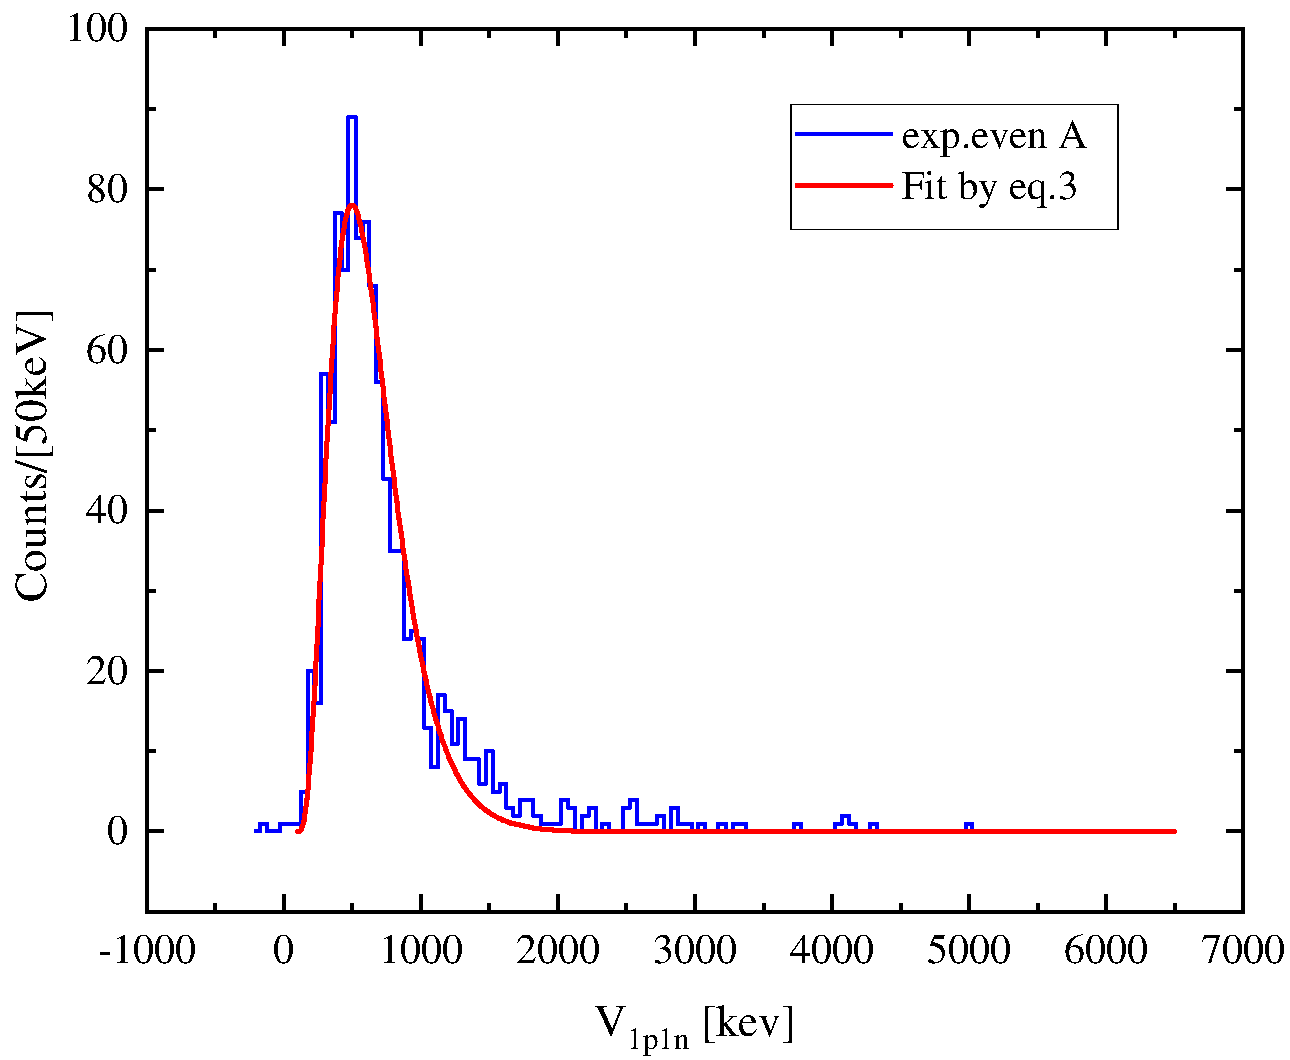
\includegraphics[width=0.4\textwidth]{figure/YE3fiteeA50.pdf}}
\qquad
\subfigure[利用公式\ref{Yukawa2}对AME2016的奇A核的$V_{1p-1n}(Z,N)$相互作用进行的拟合.\label{fig_Y3FitoA50}]{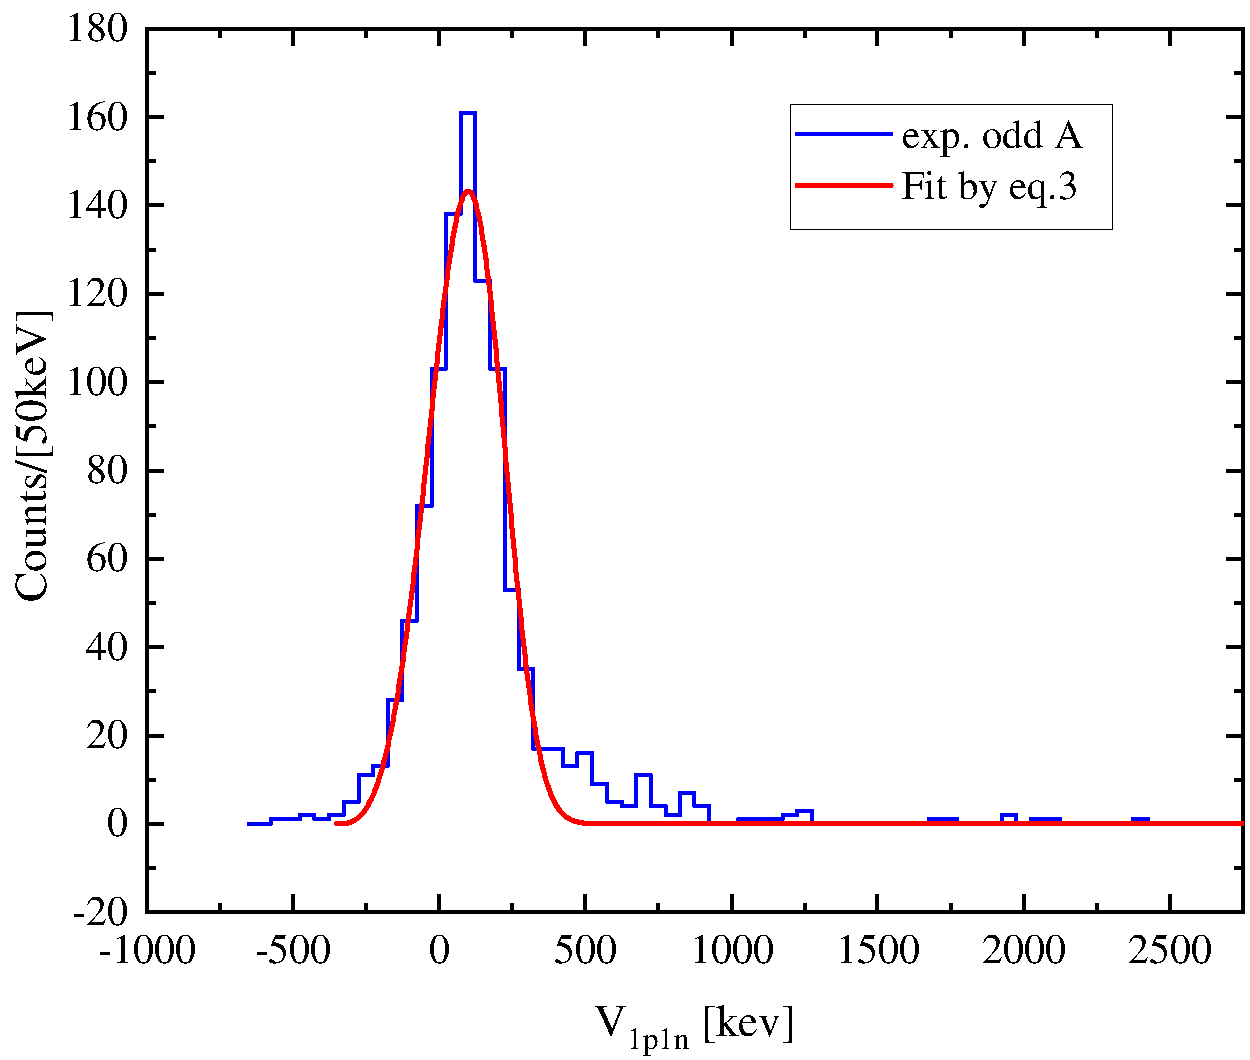
\includegraphics[width=0.4\textwidth]{figure/YE3fiteoA50.pdf}}
\caption{利用公式\ref{Yukawa2}对AME2016的$V_{1p-1n}(Z,N)$相互作用的统计分布进行的拟合.\label{fig_Y3Fit}}
\end{figure}
\section{2019.08.23}
今天的主要工作是继续对$V_{1p-1n}(Z,N)$相互作用的统计分布进行的拟合,包括对FRDM模型$V_{1p-1n}(Z,N)$~相互作用的统计分布结果的拟合,图\ref{fig_YE3FRDMFit};以及对~AME2016~的$V_{1p-1n}(Z,N)$~相互作用的统计分布结果的拟合,图\ref{fig_YE3FitV1p2n_1}及图\ref{fig_YE3FitV1p2n_1}。
\begin{figure}[H]
\centering
\subfigure[利用公式\ref{Yukawa2}对FRDM模型的偶A核的$V_{1p-1n}(Z,N)$相互作用进行的拟合.\label{fig_Y3FitFRDMeA50}]{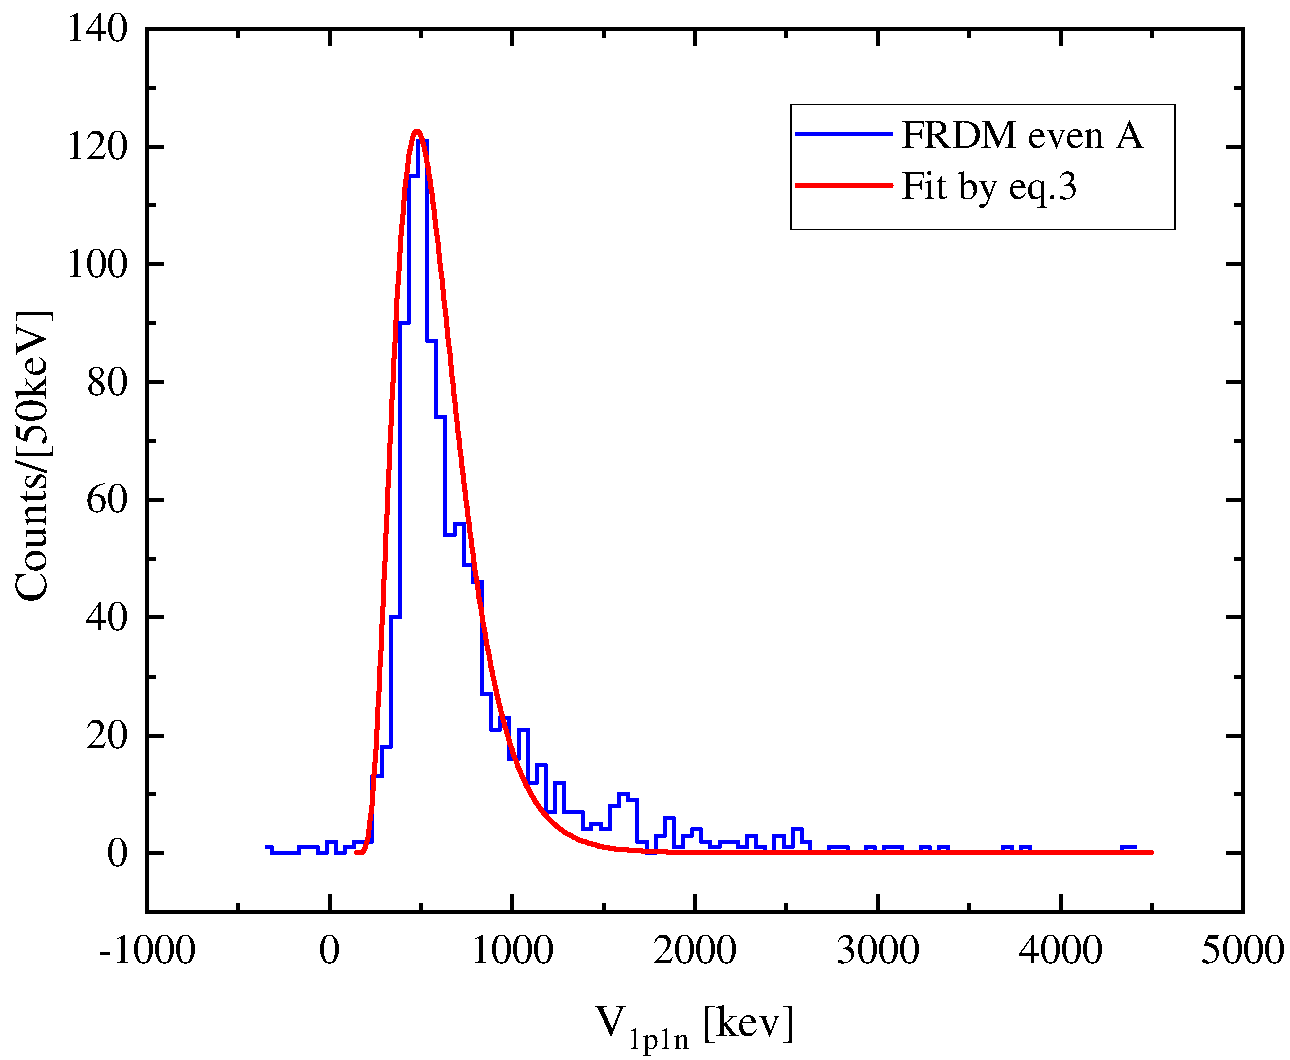
\includegraphics[width=0.4\textwidth]{figure/YE3fitFRDMoA50.pdf}}
\qquad
\subfigure[利用公式\ref{Yukawa2}对FRDM模型的奇A核的$V_{1p-1n}(Z,N)$相互作用进行的拟合.\label{fig_Y3FitFRDMoA50}]{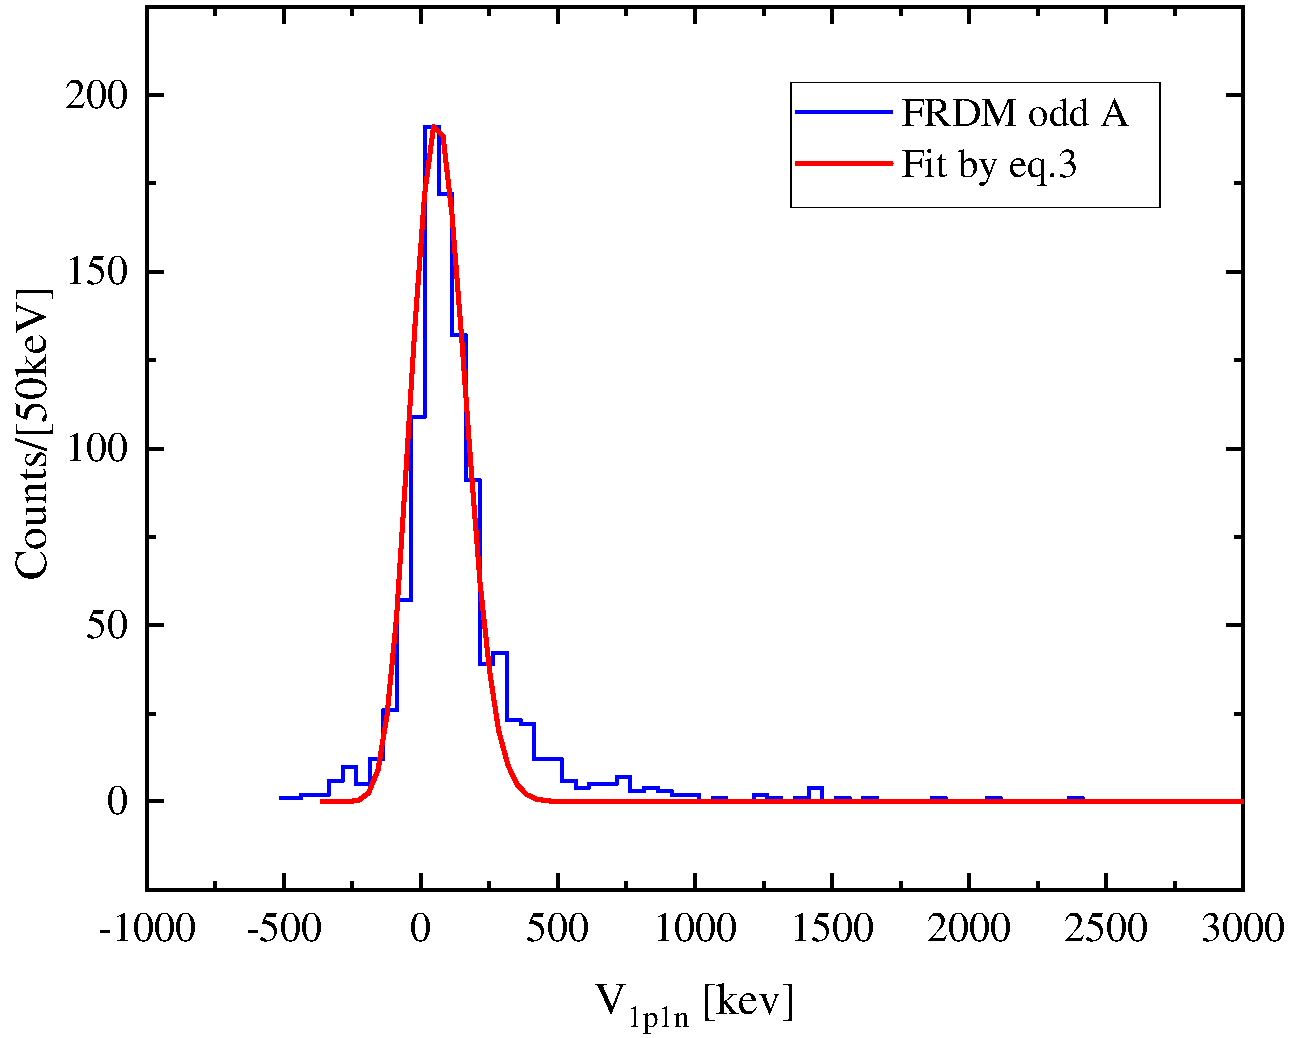
\includegraphics[width=0.4\textwidth]{figure/YE3fitFRDMeA50.pdf}}
\caption{利用公式\ref{Yukawa2}对FRDM模型的$V_{1p-1n}(Z,N)$相互作用的统计分布进行的拟合.\label{fig_YE3FRDMFit}}
\end{figure}
\begin{figure}[H]
\centering
\subfigure[利用公式\ref{Yukawa2}对AME2016的偶A核的$V_{1p-2n}(Z,N)$相互作用进行的拟合.\label{fig_Y3FitV1p2neA50}]{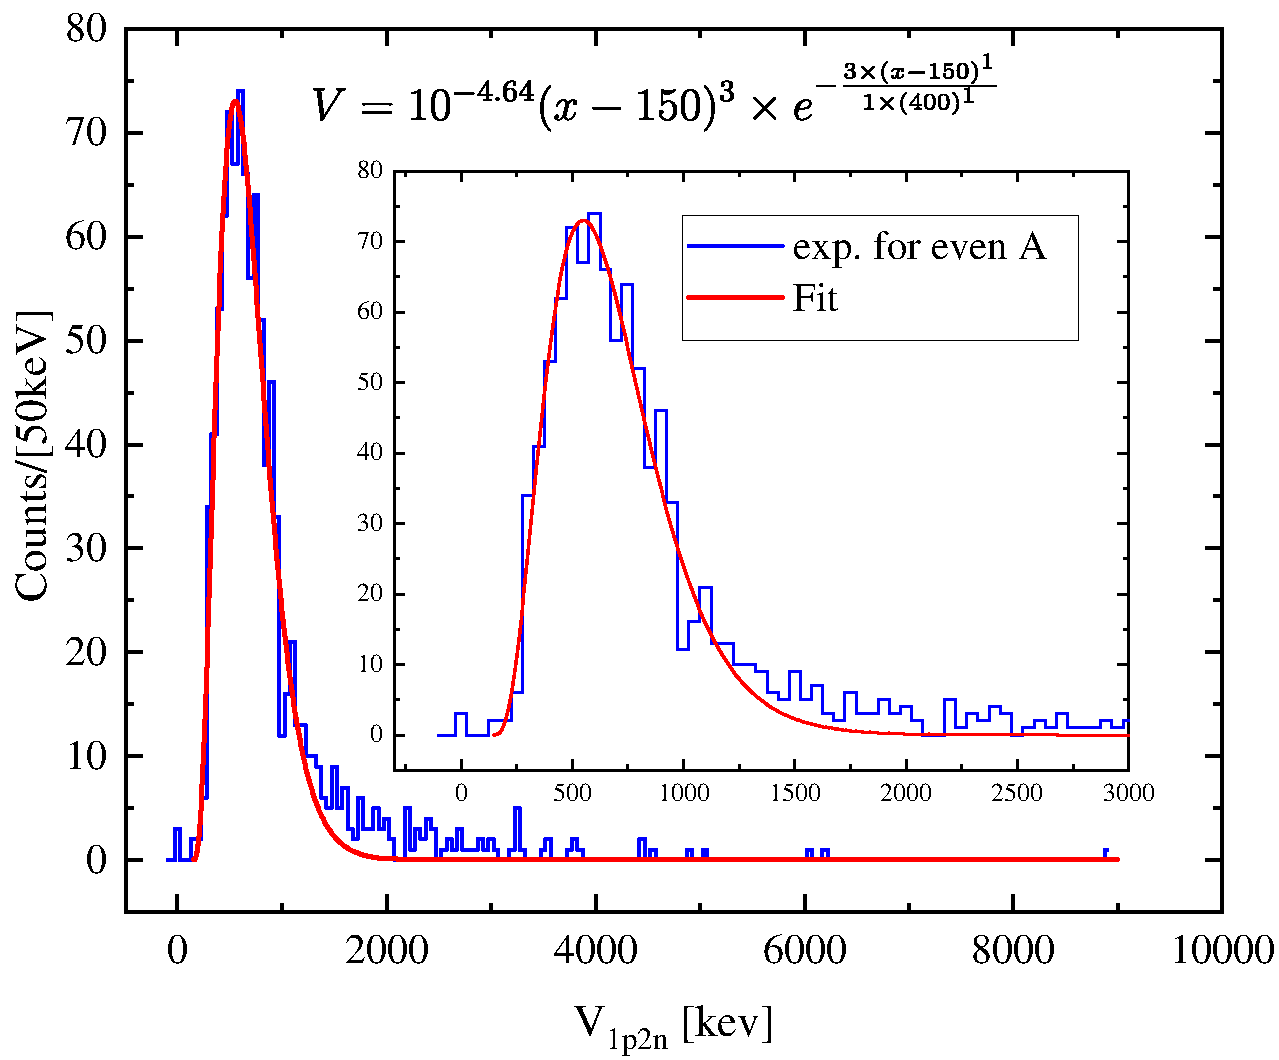
\includegraphics[width=0.4\textwidth]{figure/YE3fiteV1p2neA50.pdf}}
\qquad
\subfigure[利用公式\ref{Yukawa2}对AME2016的奇A核的$V_{1p-2n}(Z,N)$相互作用进行的拟合.\label{fig_Y3FitV1p2noA50}]{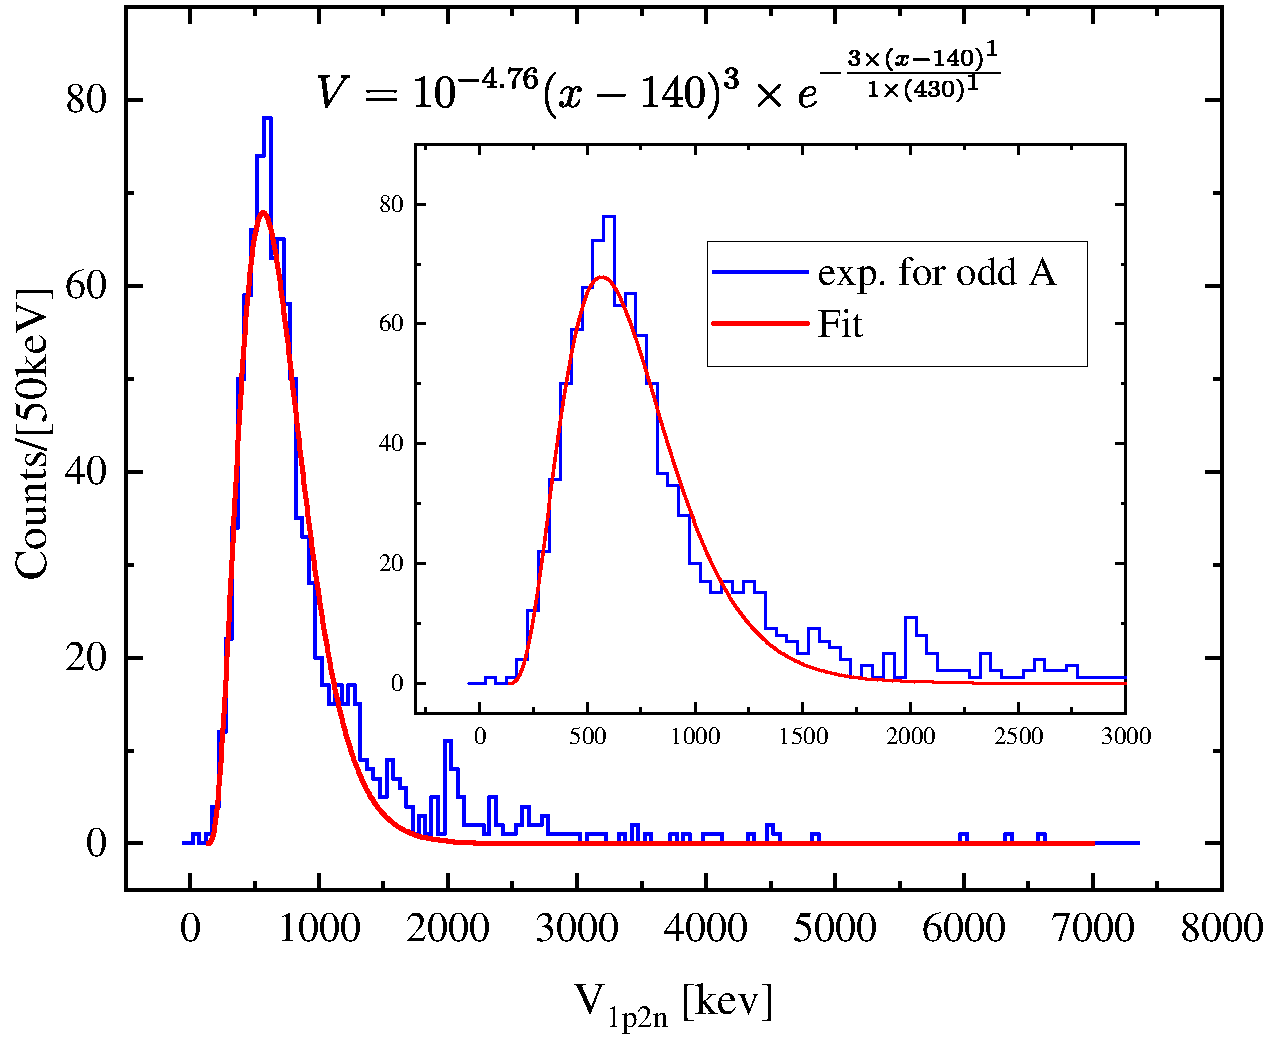
\includegraphics[width=0.4\textwidth]{figure/YE3fiteV1p2noA50.pdf}}
\caption{利用公式\ref{Yukawa2}对AME2016的$V_{1p-2n}(Z,N)$相互作用的统计分布进行的拟合.\label{fig_YE3FitV1p2n_1}}
\end{figure}
\begin{figure}[H]
\centering
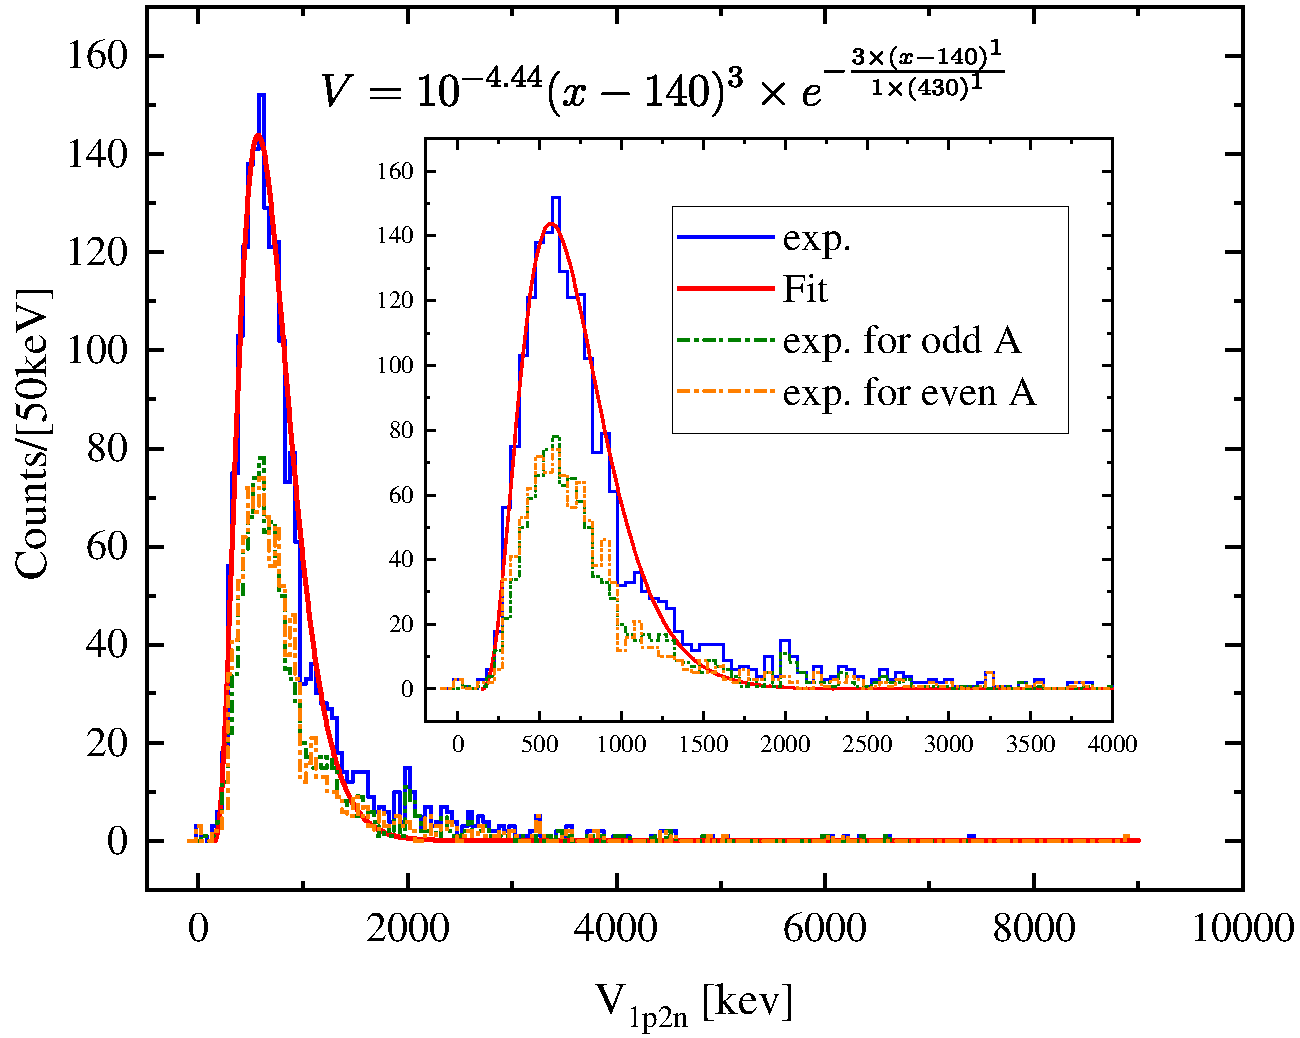
\includegraphics[width=0.6\textwidth]{YE3fiteV1p2n50.pdf}
\caption{利用公式\ref{Yukawa2}对AME2016的$V_{1p-2n}(Z,N)$相互作用整体的的统计分布进行的拟合.\label{fig_YE3FitV1p2n_2}}
\end{figure}
\section{2019.08.26}
今天的主要工作是继续对AME2016的pn相互作用的统计分布进行拟合,结果如下:
\begin{figure}[H]
\centering
\subfigure[利用公式\ref{Yukawa2}对AME2016的偶A核的$V_{2p-2n}(Z,N)$相互作用进行的拟合.\label{fig_Y3FitV2p2neA100}]{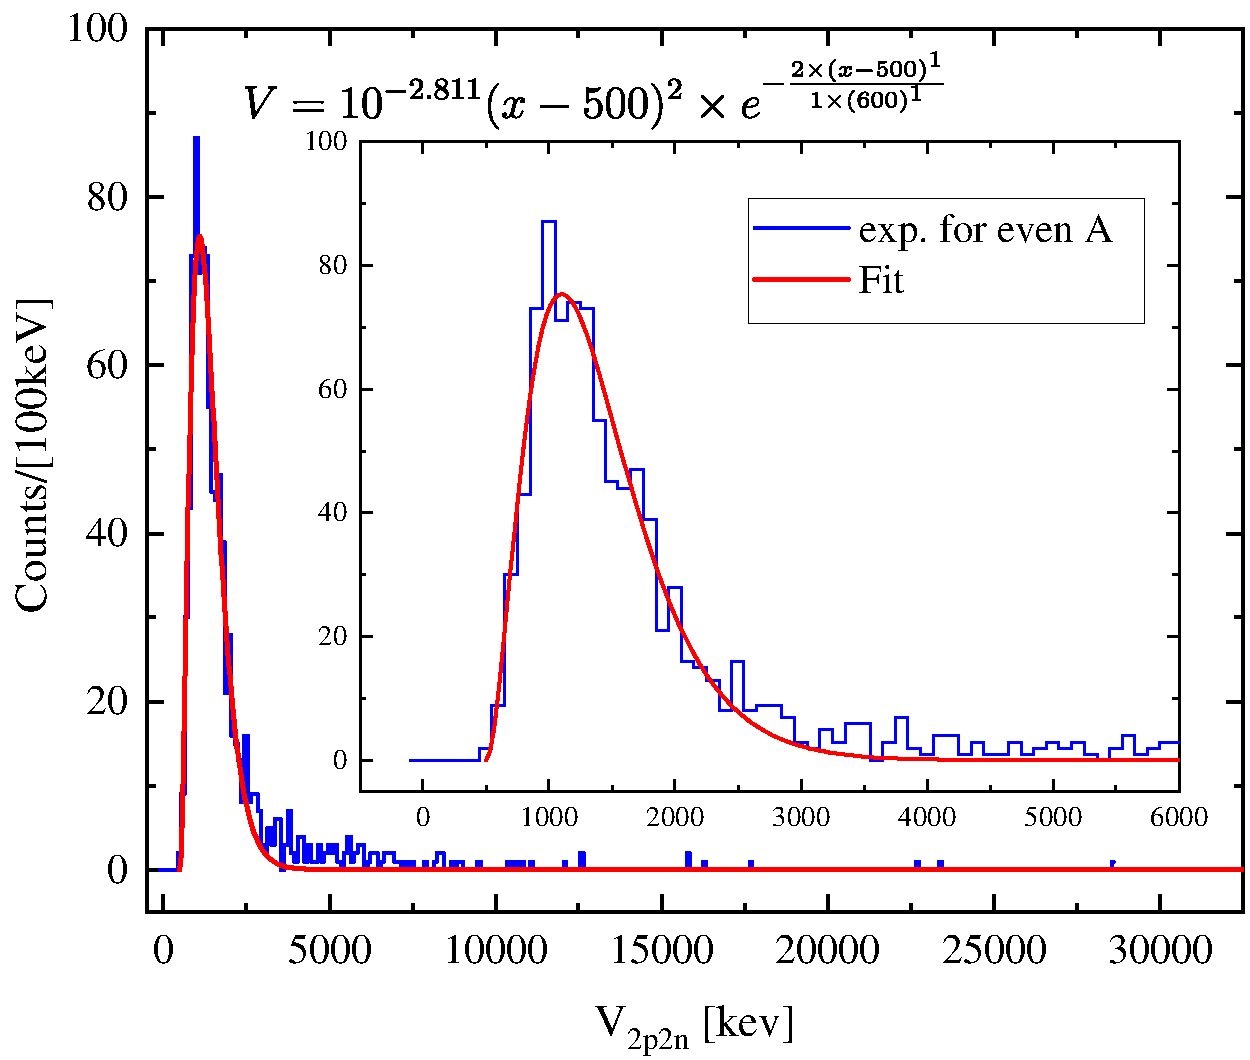
\includegraphics[width=0.4\textwidth]{figure/YE3fiteV2p2neA100.pdf}}
\qquad
\subfigure[利用公式\ref{Yukawa2}对AME2016的奇A核的$V_{2p-2n}(Z,N)$相互作用进行的拟合.\label{fig_Y3FitV2p2noA100}]{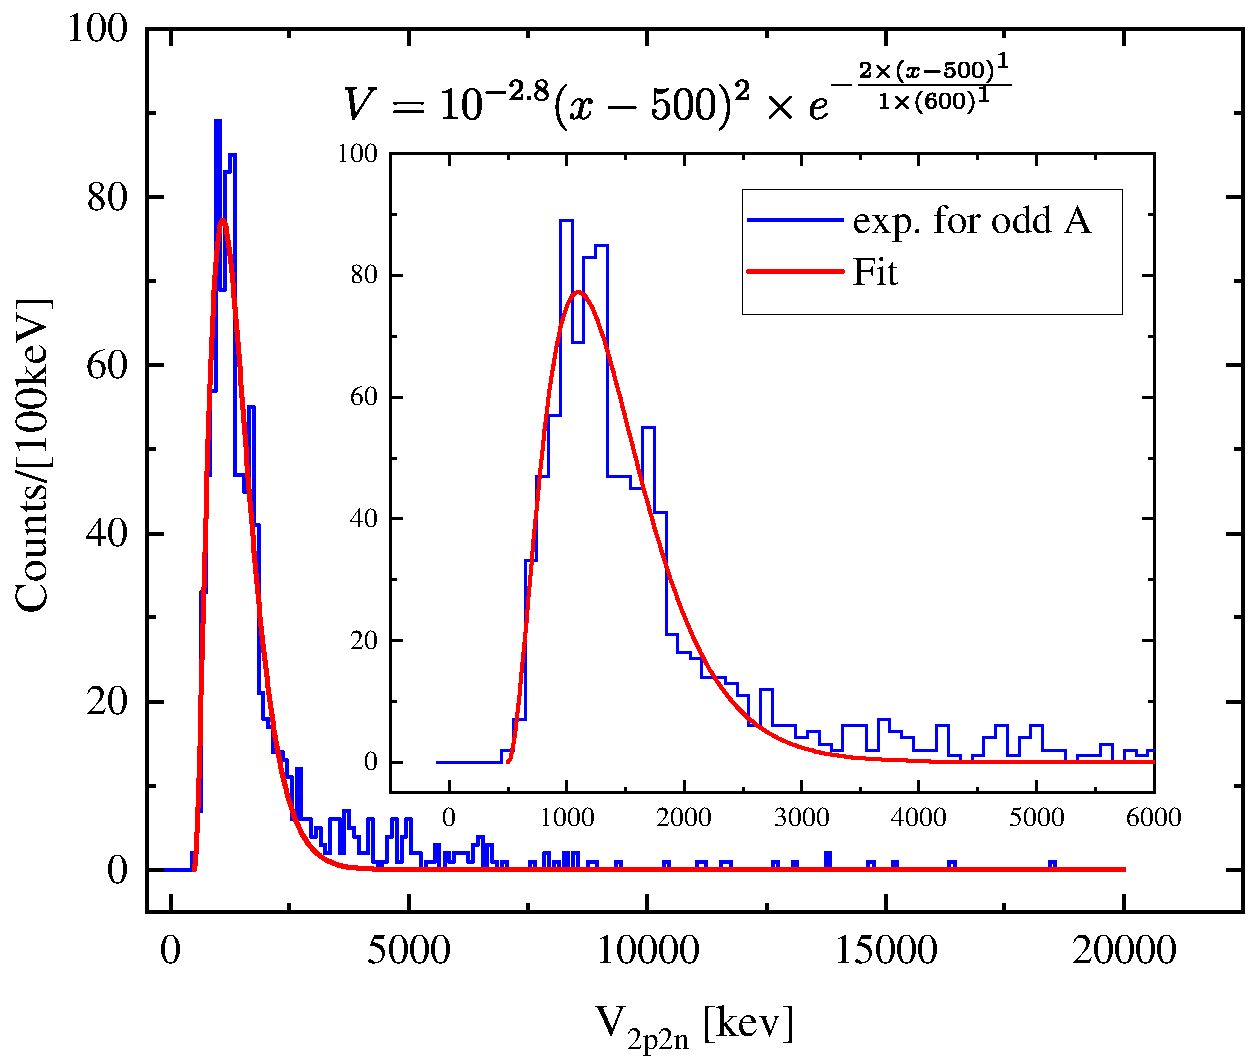
\includegraphics[width=0.4\textwidth]{figure/YE3fiteV2p2noA100.pdf}}
\caption{利用公式\ref{Yukawa2}对AME2016的$V_{2p-2n}(Z,N)$相互作用的统计分布进行的拟合.\label{fig_YE3FitV2p2n_1}}
\end{figure}
\begin{figure}[H]
\centering
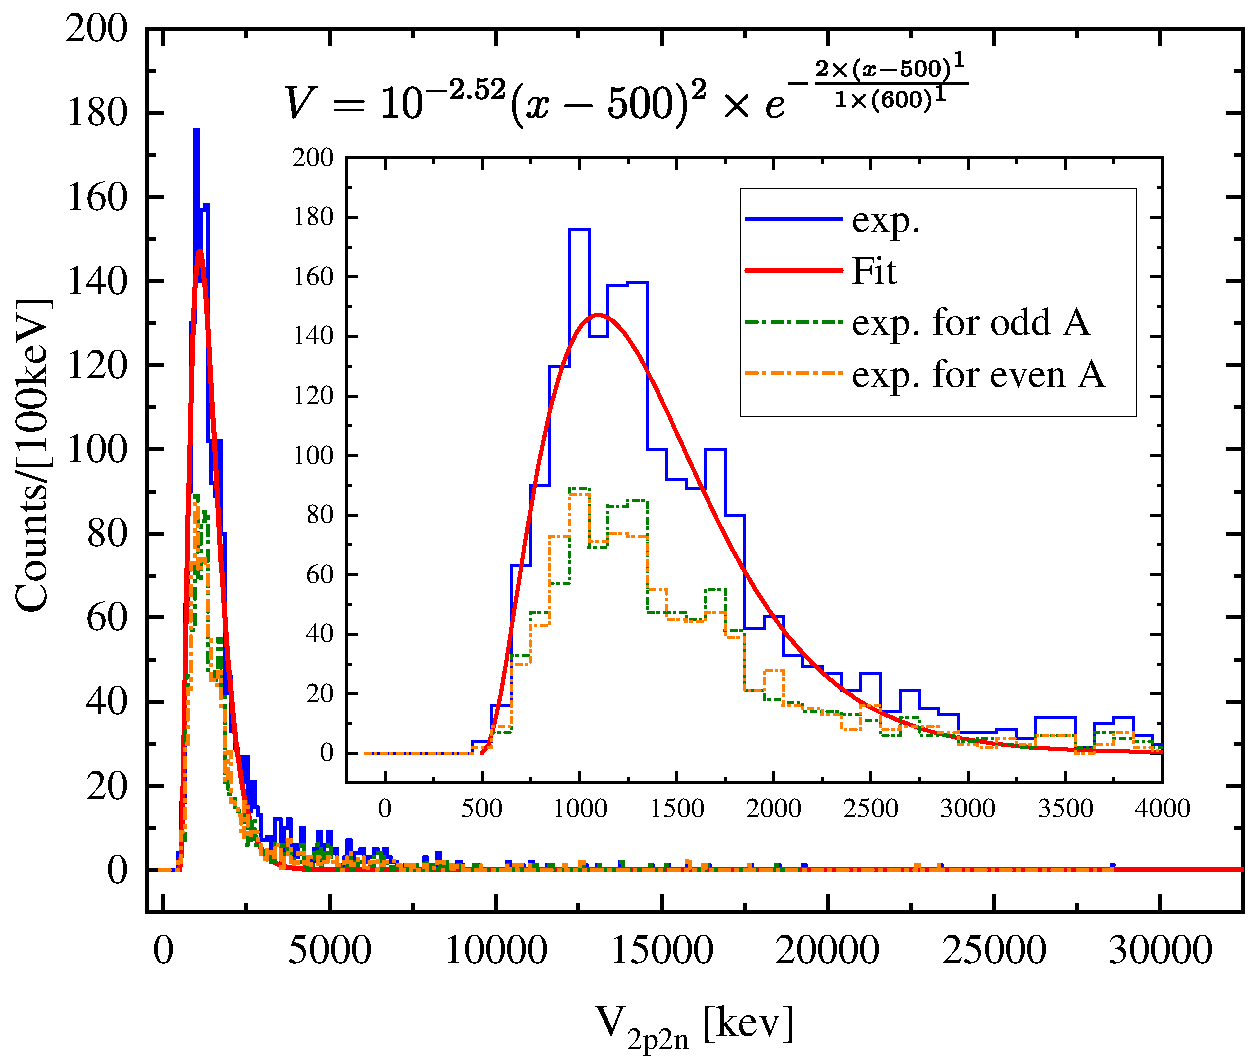
\includegraphics[width=0.6\textwidth]{YE3fiteV2p2n100.pdf}
\caption{利用公式\ref{Yukawa2}对AME2016的$V_{2p-2n}(Z,N)$相互作用整体的的统计分布进行的拟合.\label{fig_YE3FitV2p2n}}
\end{figure}
\section{2019.08.27}
今天的主要工作是继续对AME2016的pn相互作用的统计分布进行拟合,结果如下:
\begin{figure}[H]
\centering
\subfigure[利用公式\ref{Yukawa2}对AME2016的偶A核的$V_{1p-3n}(Z,N)$相互作用进行的拟合.\label{fig_Y3FitV1p3neA100}]{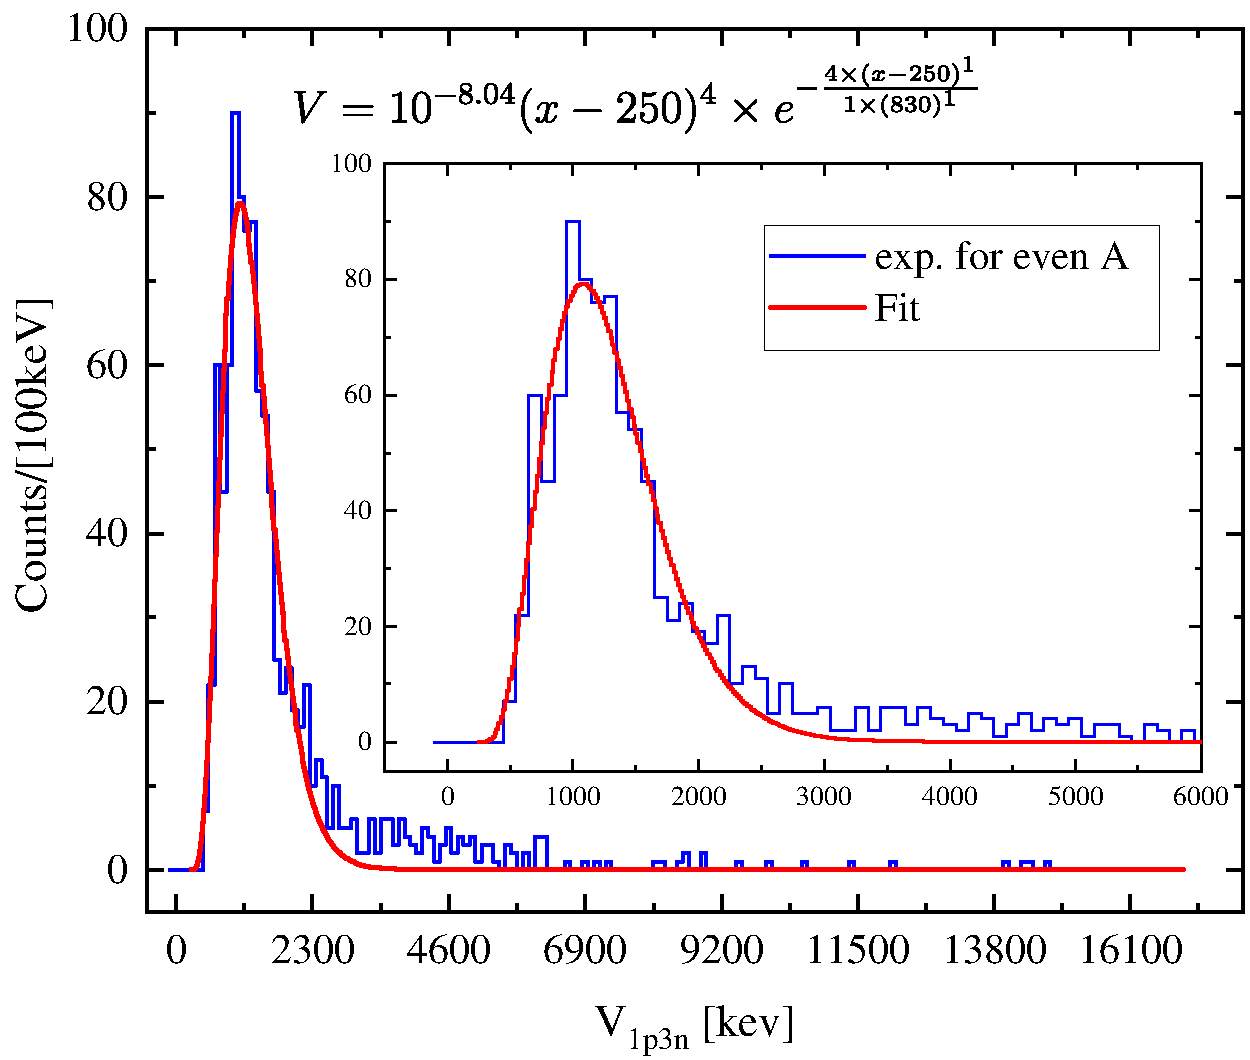
\includegraphics[width=0.4\textwidth]{figure/YE3fiteV1p3neA100.pdf}}
\qquad
\subfigure[利用公式\ref{Yukawa2}对AME2016的奇A核的$V_{1p-3n}(Z,N)$相互作用进行的拟合.\label{fig_Y3FitV1p3noA100}]{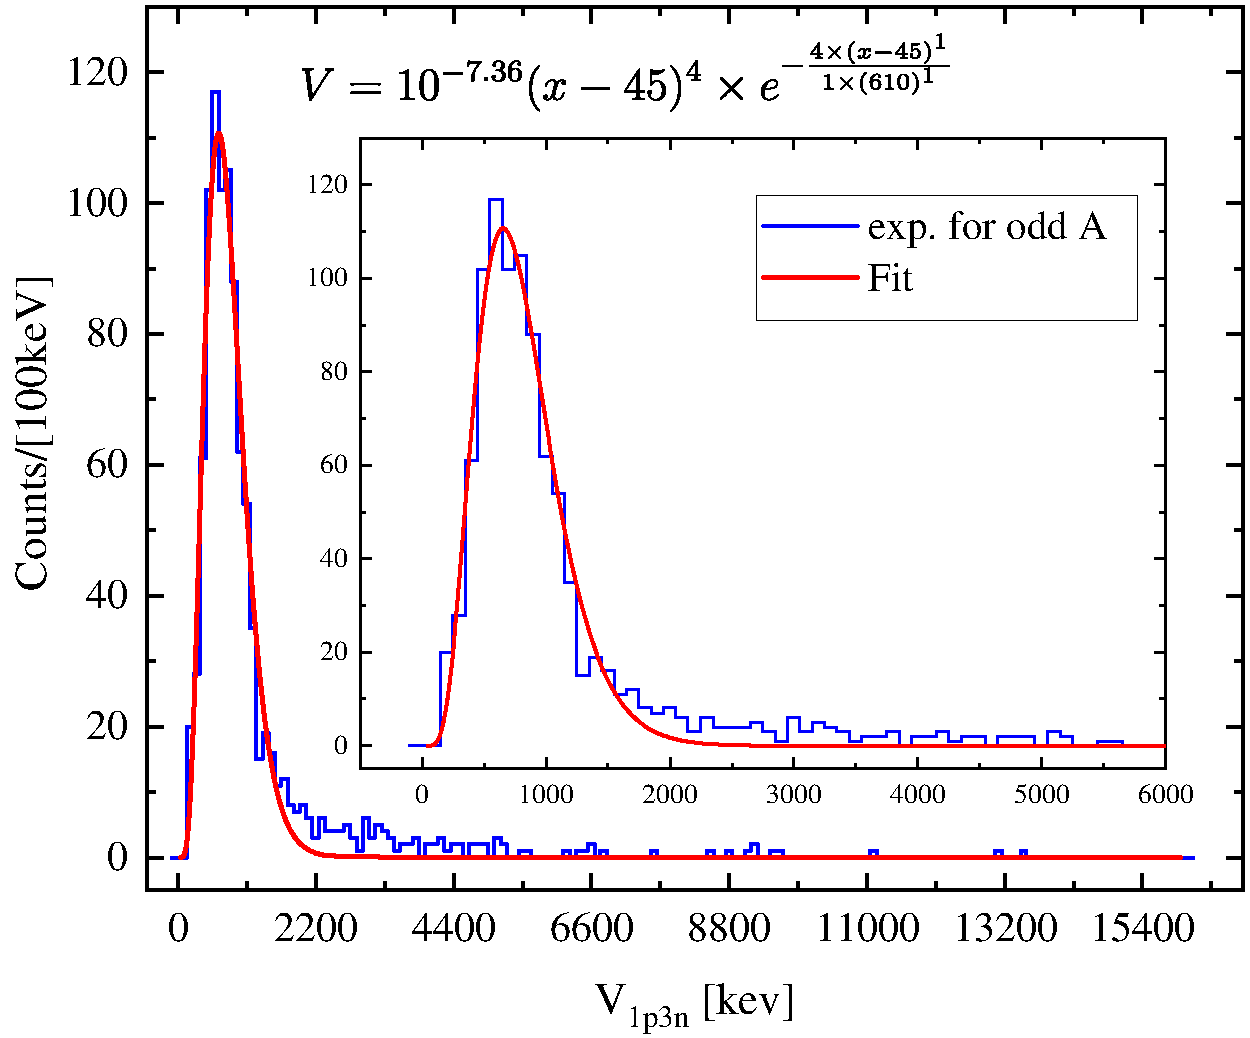
\includegraphics[width=0.4\textwidth]{figure/YE3fiteV1p3noA100.pdf}}
\caption{利用公式\ref{Yukawa2}对AME2016的$V_{1p-3n}(Z,N)$相互作用的统计分布进行的拟合.\label{fig_YE3FitV1p3n_1}}
\end{figure}
\begin{figure}[H]
\centering
\subfigure[利用公式\ref{Yukawa2}对AME2016的偶A核的$V_{3p-1n}(Z,N)$相互作用进行的拟合.\label{fig_Y3FitV3p1neA100}]{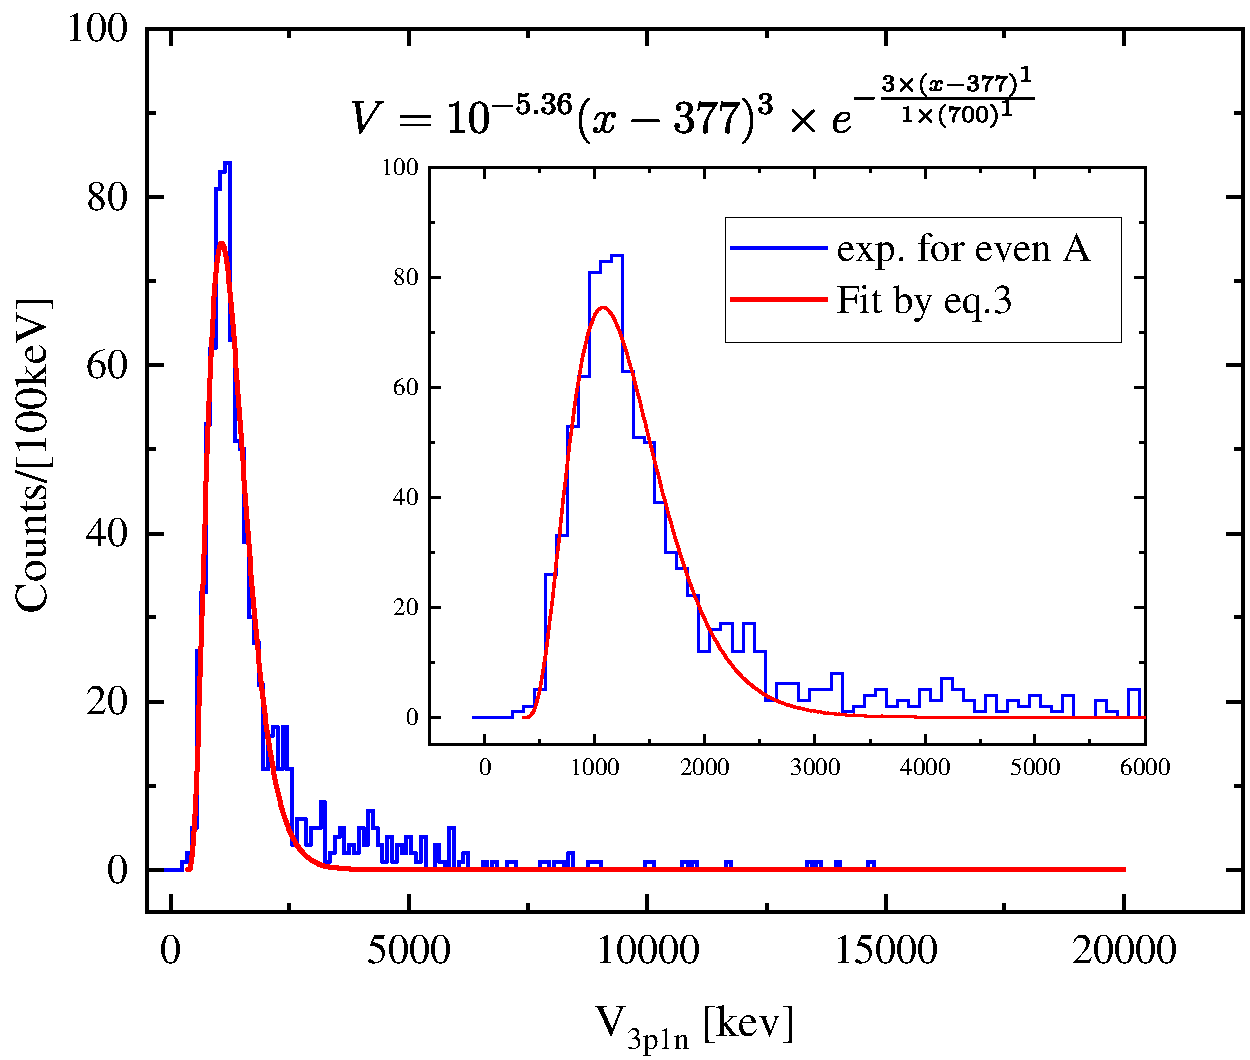
\includegraphics[width=0.4\textwidth]{figure/YE3fiteV3p1neA100.pdf}}
\qquad
\subfigure[利用公式\ref{Yukawa2}对AME2016的奇A核的$V_{3p-1n}(Z,N)$相互作用进行的拟合.\label{fig_Y3FitV3p1noA100}]{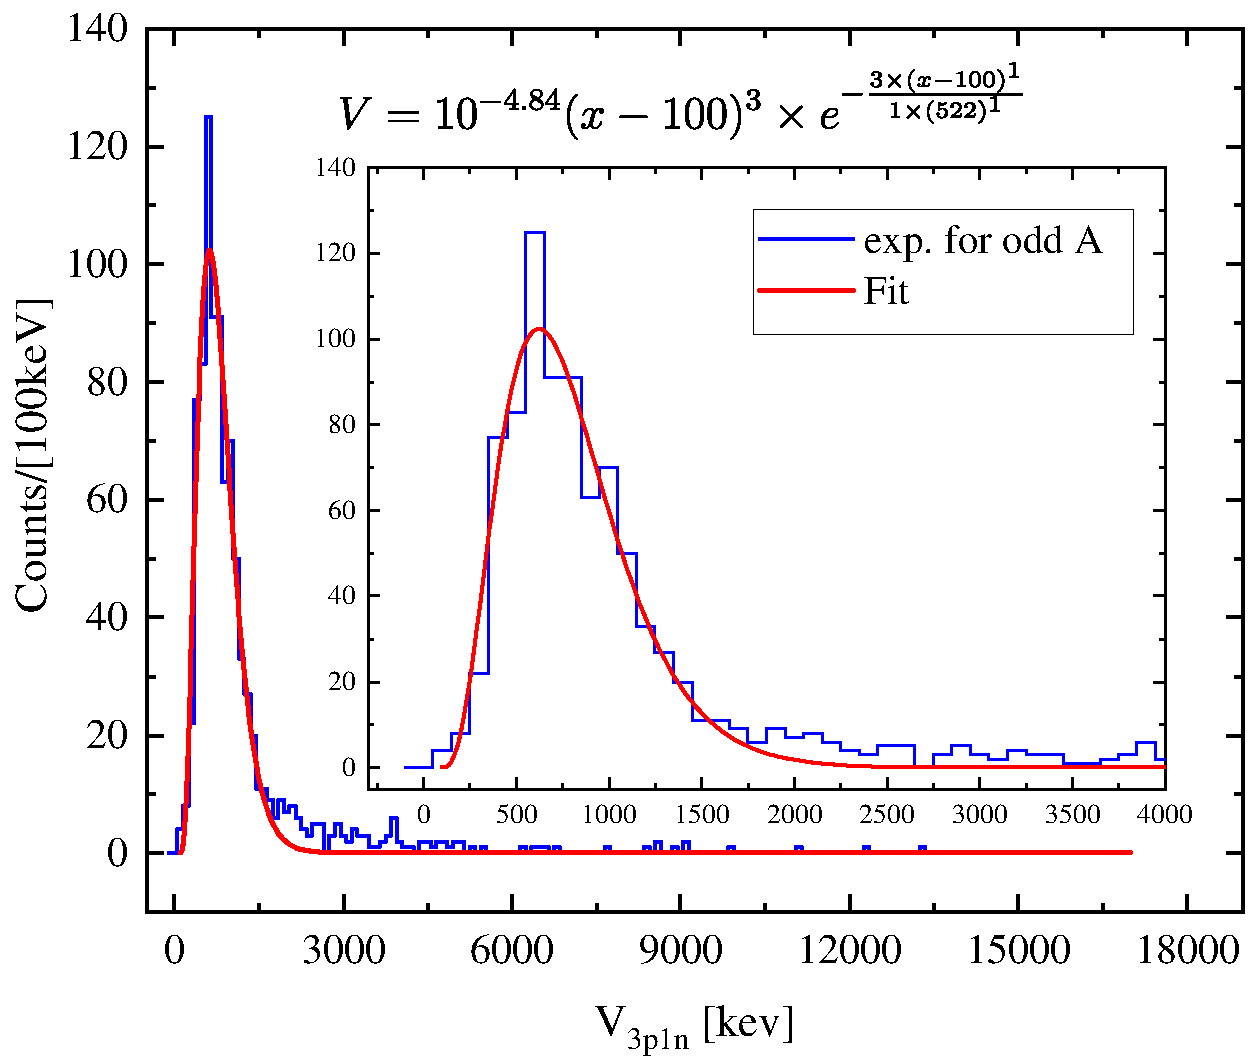
\includegraphics[width=0.4\textwidth]{figure/YE3fiteV3p1noA100.pdf}}
\caption{利用公式\ref{Yukawa2}对AME2016的$V_{3p-1n}(Z,N)$相互作用的统计分布进行的拟合.\label{fig_YE3FitV1p3n_1}}
\end{figure}
\section{2019.08.28}
今天的主要工作是继续对AME2016的最外层质子对和中子对相互作用$V_{Pp}(Z,N)$、$V_{Pn}(Z,N)$的统计分布进行拟合,结果如下:
\begin{figure}[H]
\centering
\subfigure[利用公式\ref{Yukawa2}对AME2016的偶Z核的$V_{Pp}(Z,N)$相互作用进行的拟合.\label{fig_Y3FitVPp100}]{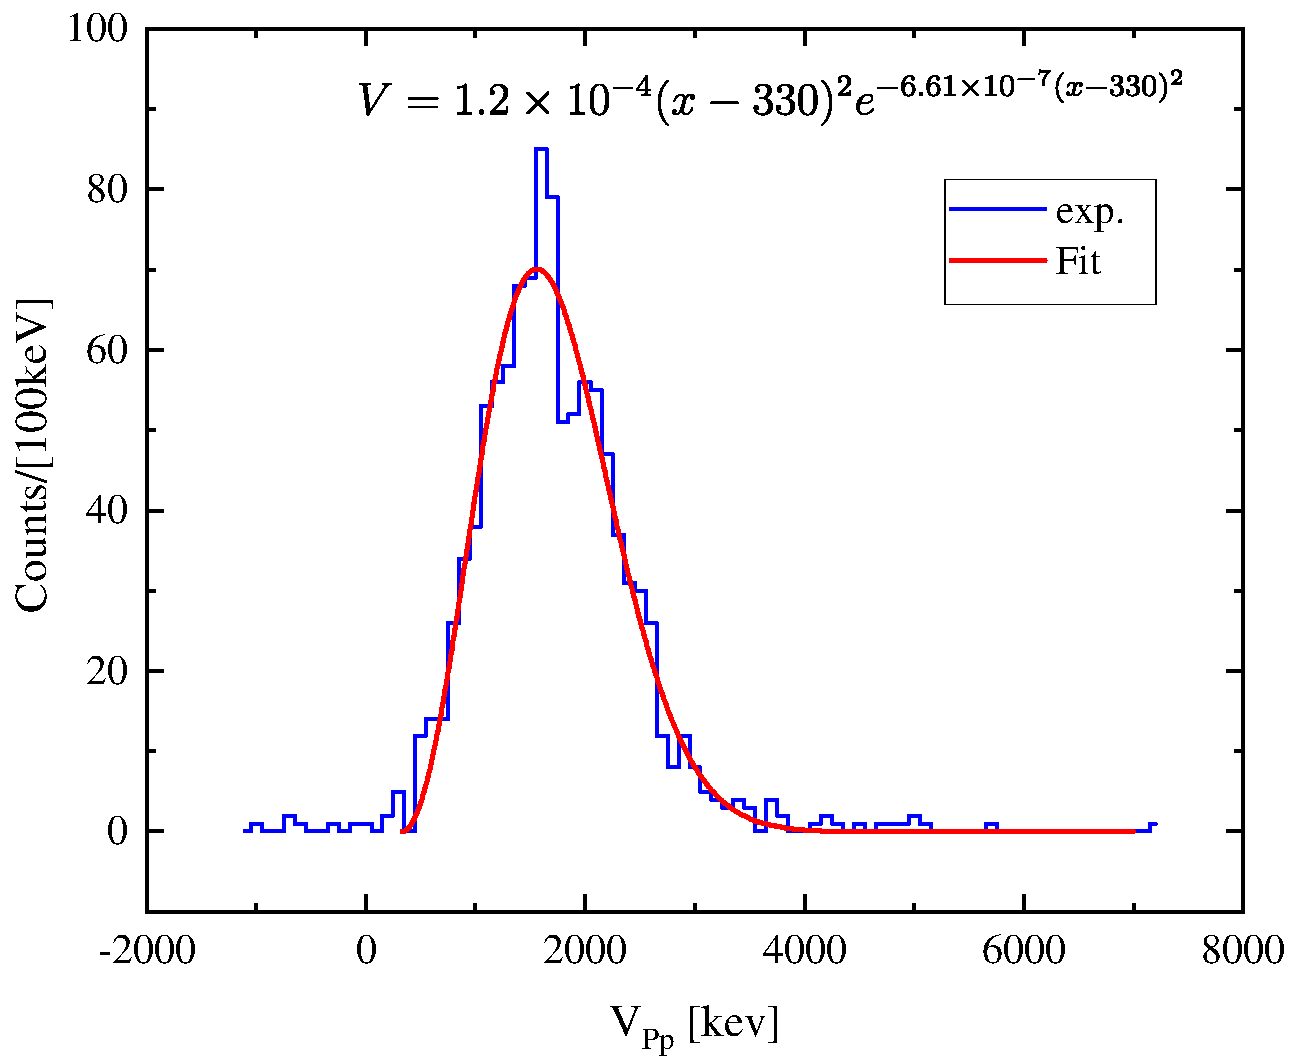
\includegraphics[width=0.4\textwidth]{figure/YE3fiteVPp100.pdf}}
\qquad
\subfigure[利用公式\ref{Yukawa2}对AME2016的偶N核的$V_{Pn}(Z,N)$相互作用进行的拟合.\label{fig_Y3FitVPn100}]{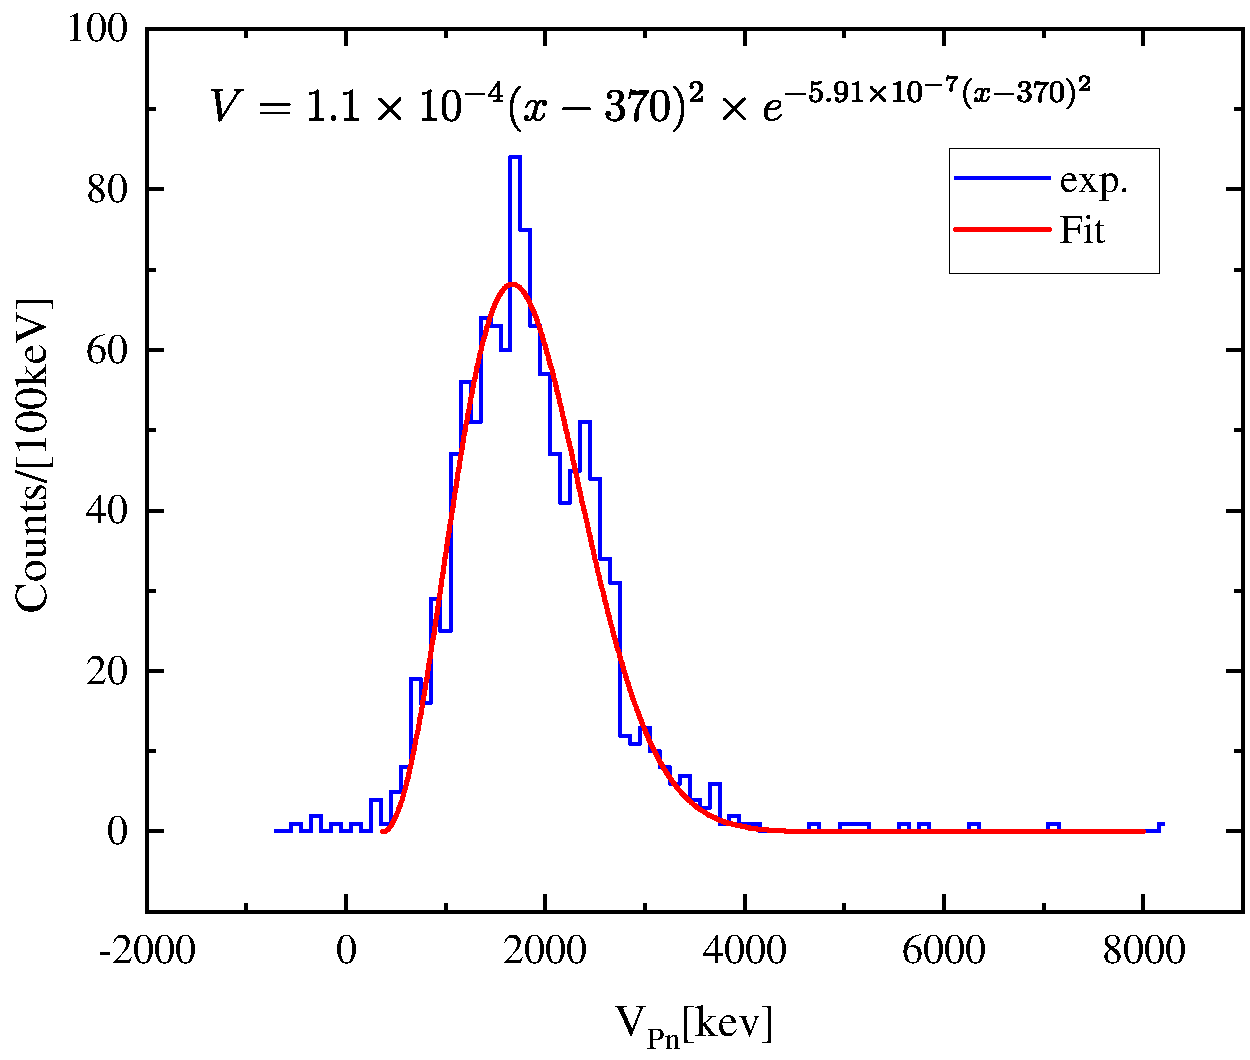
\includegraphics[width=0.4\textwidth]{figure/YE3fiteVPn100.pdf}}
\caption{利用公式\ref{Yukawa2}对AME2016的$V_{3p-1n}(Z,N)$相互作用的统计分布进行的拟合.\label{fig_YE3FitV1p3n_1}}
\end{figure}
\section{2019.08.29}
今天的主要工作是完成上学期原子核结构和核天体物理两门课程的试卷。
\section{2019.08.30}
今天的主要工作是完成昨天没有写完的原子核结构试卷和实验数据分析的课的试卷。
\section{2019.08.31}
今天的主要工作是准备原子核结构和核天体物理两门课程的报告的ppt。
\section{2019.09.01}
今天准备重复一篇Phys. Rev. Lett. 文章\href{https://journals.aps.org/prl/abstract/10.1103/PhysRevLett.119.252501}{<Estimating Parameter Uncertainty in Binding-Energy Models by the Frequency-Domain Bootstrap>}的内容。这篇文章主要介绍了三种的得到模型参数的不确定性的方法包括$\chi^2$方法、bootstrap方法和frequency-domain bootstrap (FDB)。

\section{2019.09.02}
今天为了重复参考文献\cite{RN569},寻找并阅读了相关的文献\cite{RN572,RN570},此外还找到了在文献\cite{RN569}中需要使用的AME2003的数据(如图\ref{PERAME2003}所示),并与AME2016做了对比,蓝色的代表AME2016中新增的通过实验测得了质量的核素,
\begin{figure}[H]
\centering
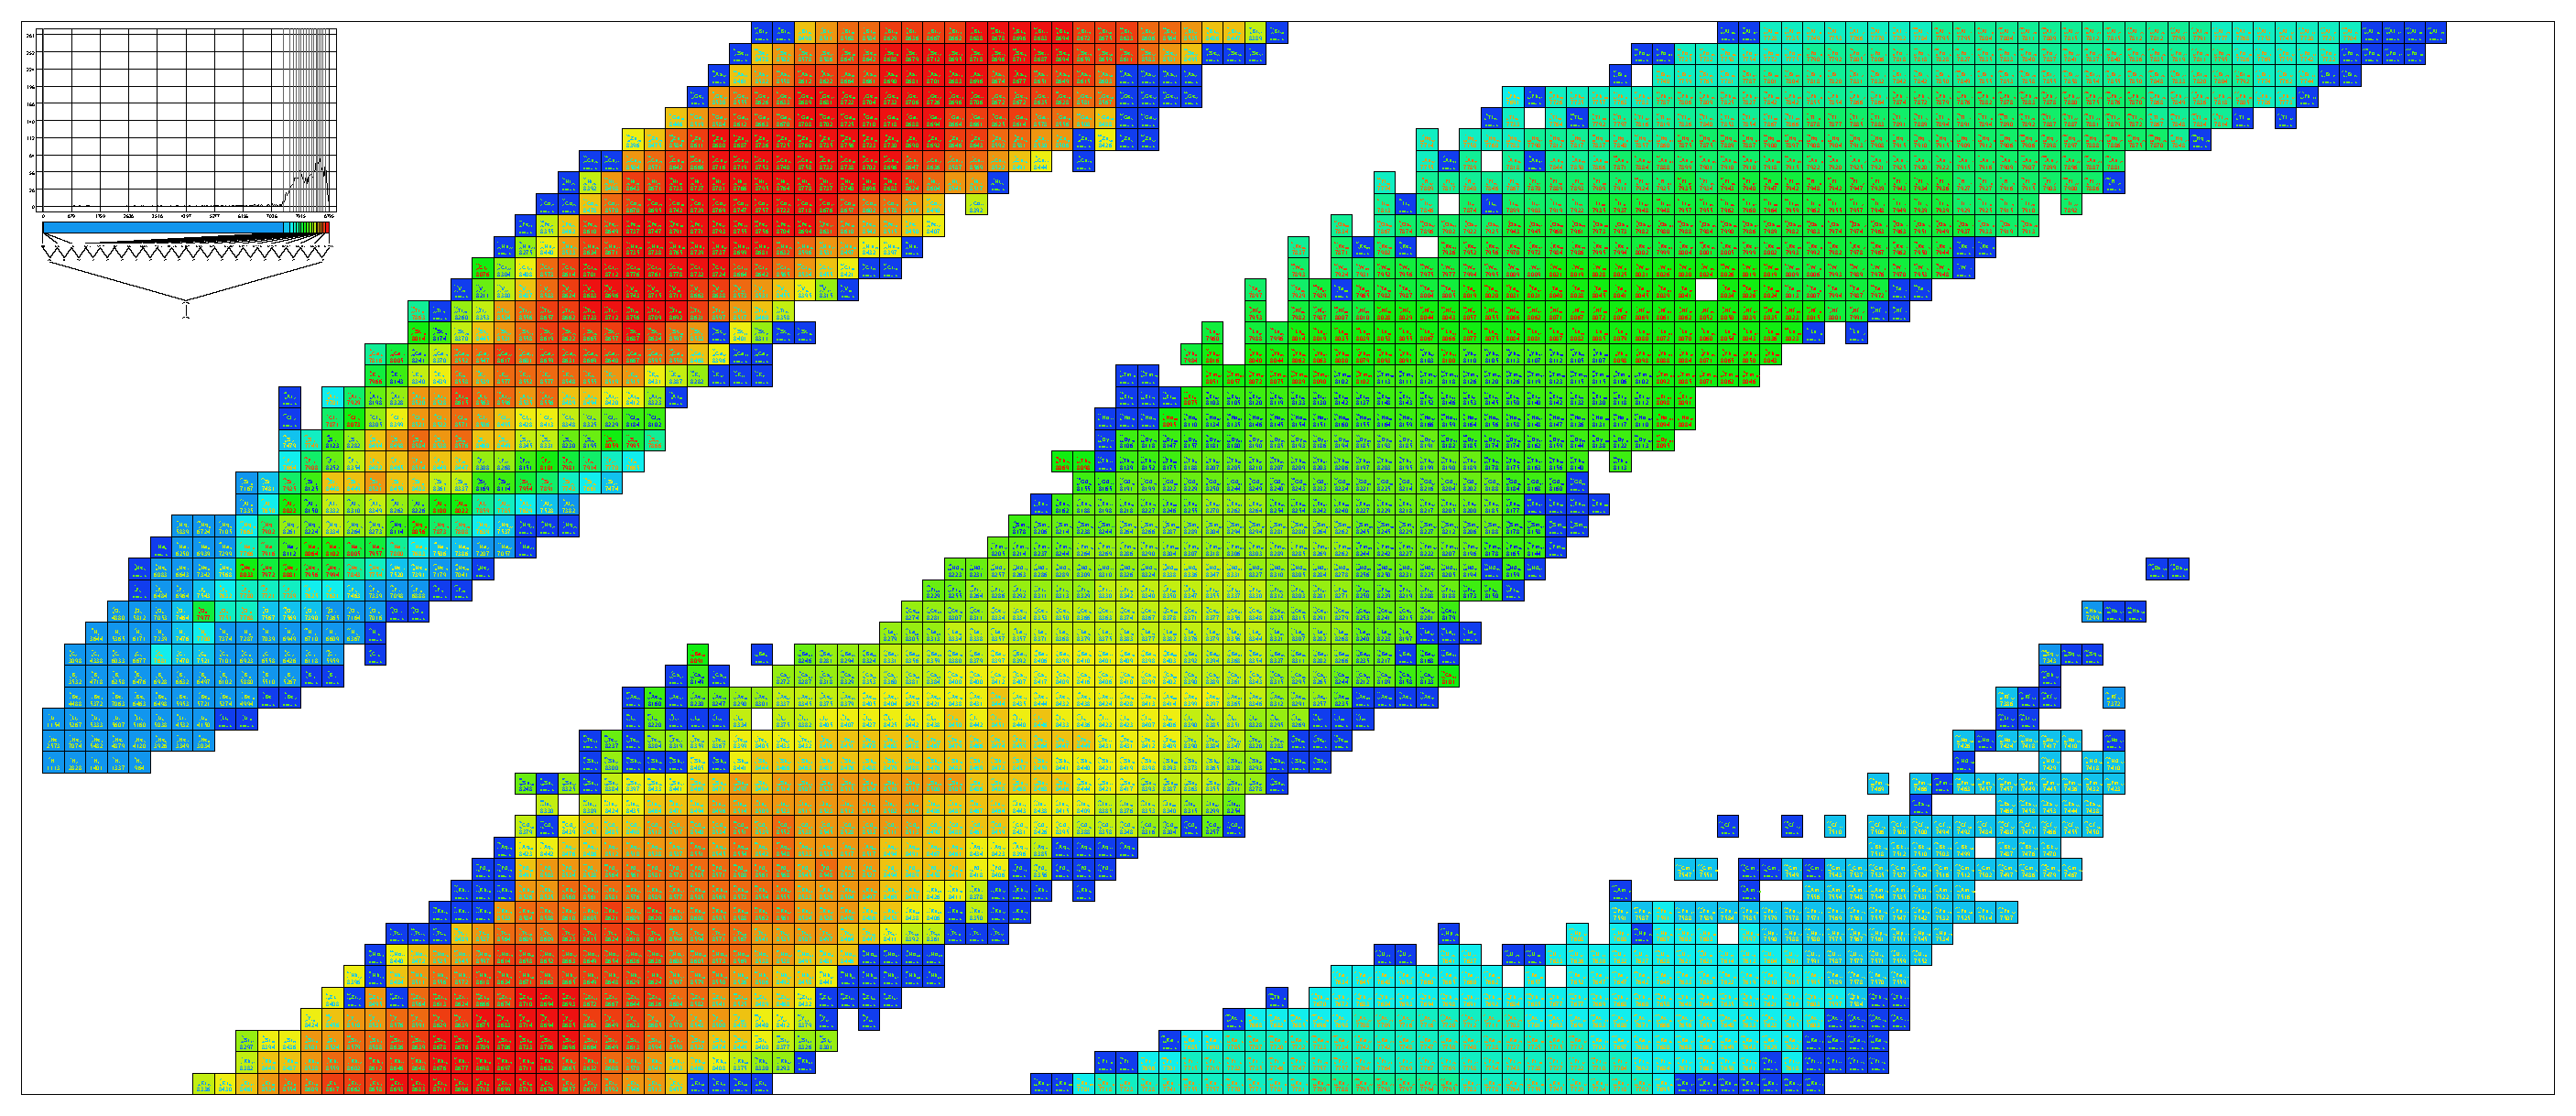
\includegraphics[width=0.9\textwidth]{PERAME2003.pdf}
\caption{AME2003质量表中所有实验已知的核素的比结合能(蓝色的代表AME2016中新增的通过实验测得了质量的核素).\label{PERAME2003}}
\end{figure}

\section{2019.09.03}
今天重复了文献\cite{RN569}中的$\chi^2$方法,在文献\cite{RN569}中液滴模型使用的参数是$a_v=15.58$MeV、$a_sym=22.18$MeV但是文章中并没有给出其他的参数,也没有给出其引用的相应的参考文献,所以我们在这里所使用的液滴模型是在卢希庭的书中给出的:
\begin{eqnarray*}
    B(Z,A)&=&B_v+B_s+B_c+B_{sym}+B_p\\
    &=&a_vA-a_sA^{2/3}-a_cZ^2A^{-1/3}-a_{sym}\left(\frac{A}{2}-Z\right)^2A^{-1}+a_p\delta A^{-1/2}
\end{eqnarray*}
其中$B_p$项为:
\begin{displaymath}
B_p= \left\{ \begin{array}{ll}
a_pA^{-1/2}& \textrm{偶偶核}\\
0 & \textrm{奇A核}\\
-a_pA^{-1/2} & \textrm{奇奇核}
\end{array} \right.
\end{displaymath}
其参量可以取值为:
其中参量可以取值为:
\begin{eqnarray*}
    a_v&=&15.835\textrm{MeV}\\
    a_s&=&18.33\textrm{MeV}\\
    a_c&=&0.714\textrm{MeV}\\
    a_{sym}&=&92.80\textrm{MeV}\\
    a_p&=&11.2\textrm{MeV}\\
\end{eqnarray*}
利用其与AME2003质量表中的2000多个实验已知的核素的质量相减的残差分布如图\ref{fig_risdAME2003}。
\begin{figure}[H]
\centering
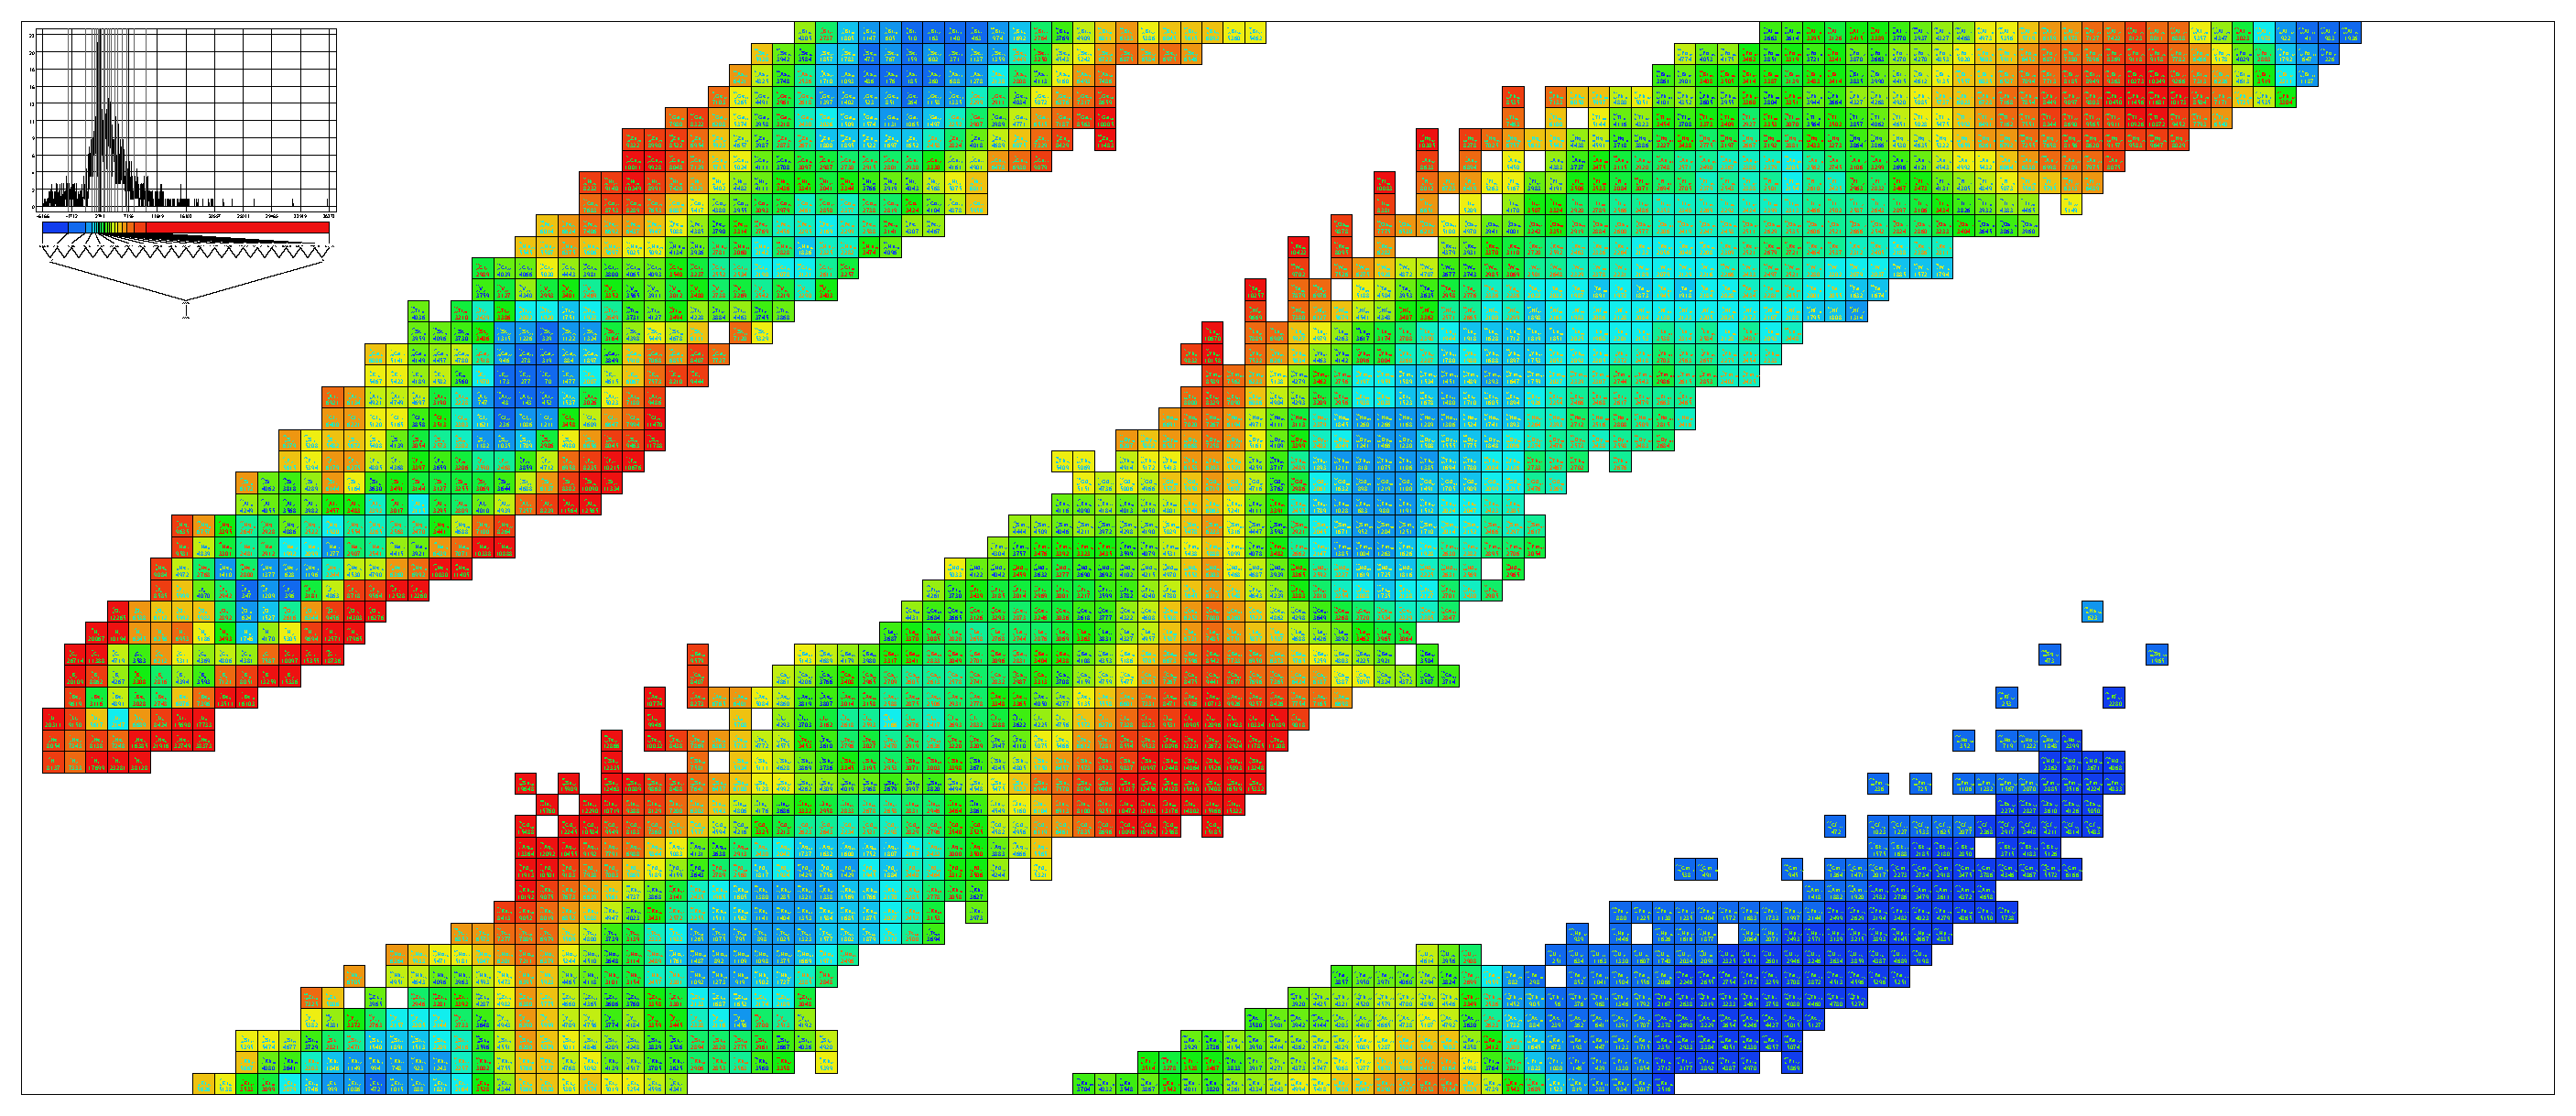
\includegraphics[width=0.9\textwidth]{risdAME2003.pdf}
\caption{液滴模型与AME2003质量表中的2000多个实验已知的核素的质量相减的残差分布.\label{fig_risdAME2003}}
\end{figure}
可以看到其与文献\cite{RN569}中FIG. 1给出的残差分布基本一致。再利用文献\cite{RN569}中的$\chi^2$方法的公式:
\begin{equation}
	L(p)=\frac{1}{(2\pi\sigma_0^2)}^{S/2}\textrm{exp}\left\{-\sum^S_{i=1}[y_\textrm{expt}(x_i)-M(x_i,p)]^2/2\sigma^2_0\right\}
\end{equation}
我们的得到的结果如图\ref{fig_chi2fit}与文献\cite{RN569}中的$\chi^2$方法的结果$a_v=15.58$MeV、$\sigma_{a_v}=0.03$基本一致。
\begin{figure}[H]
\centering
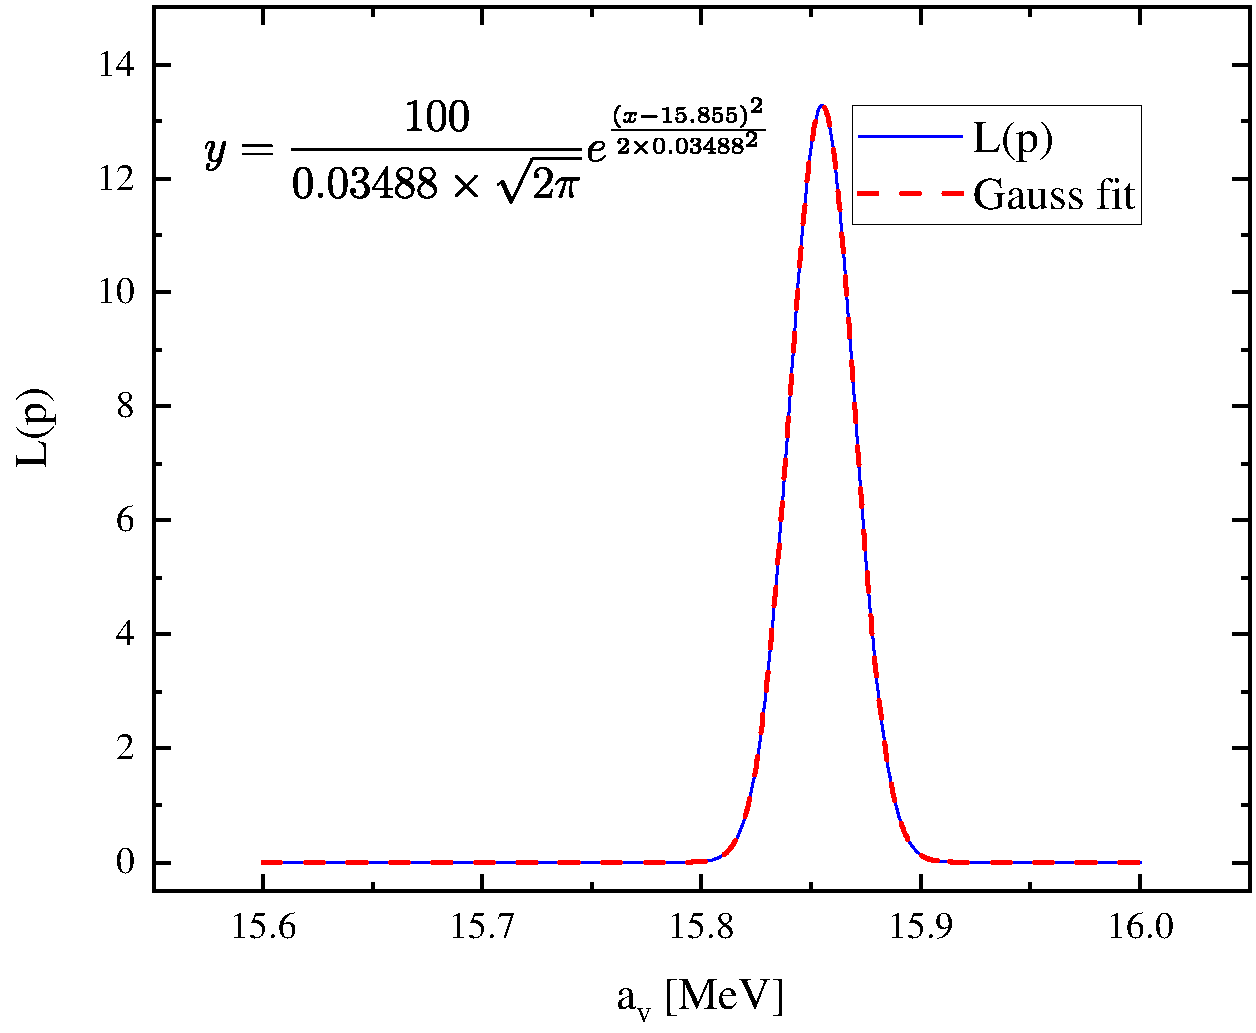
\includegraphics[width=0.6\textwidth]{chi2fit.pdf}
\caption{利用$\chi^2$方法得到的$L(a_v)$的分布,其中心值为15.855MeV,不确定度$\sigma=0.035$.\label{fig_chi2fit}}
\end{figure}

\section{2019.09.04}
今天在重复文献\cite{RN569}中的uncorrelated bootstrap(UCB)方法时,计算得到的结果如图\ref{fig_UCBAME2003},$a_v$的不确定度为0.00312 MeV,与文章中给出的0.03 MeV存在数量级的差异,目前正在查阅文章对应的参考文献\cite{RN570}。
\begin{figure}[H]
\centering
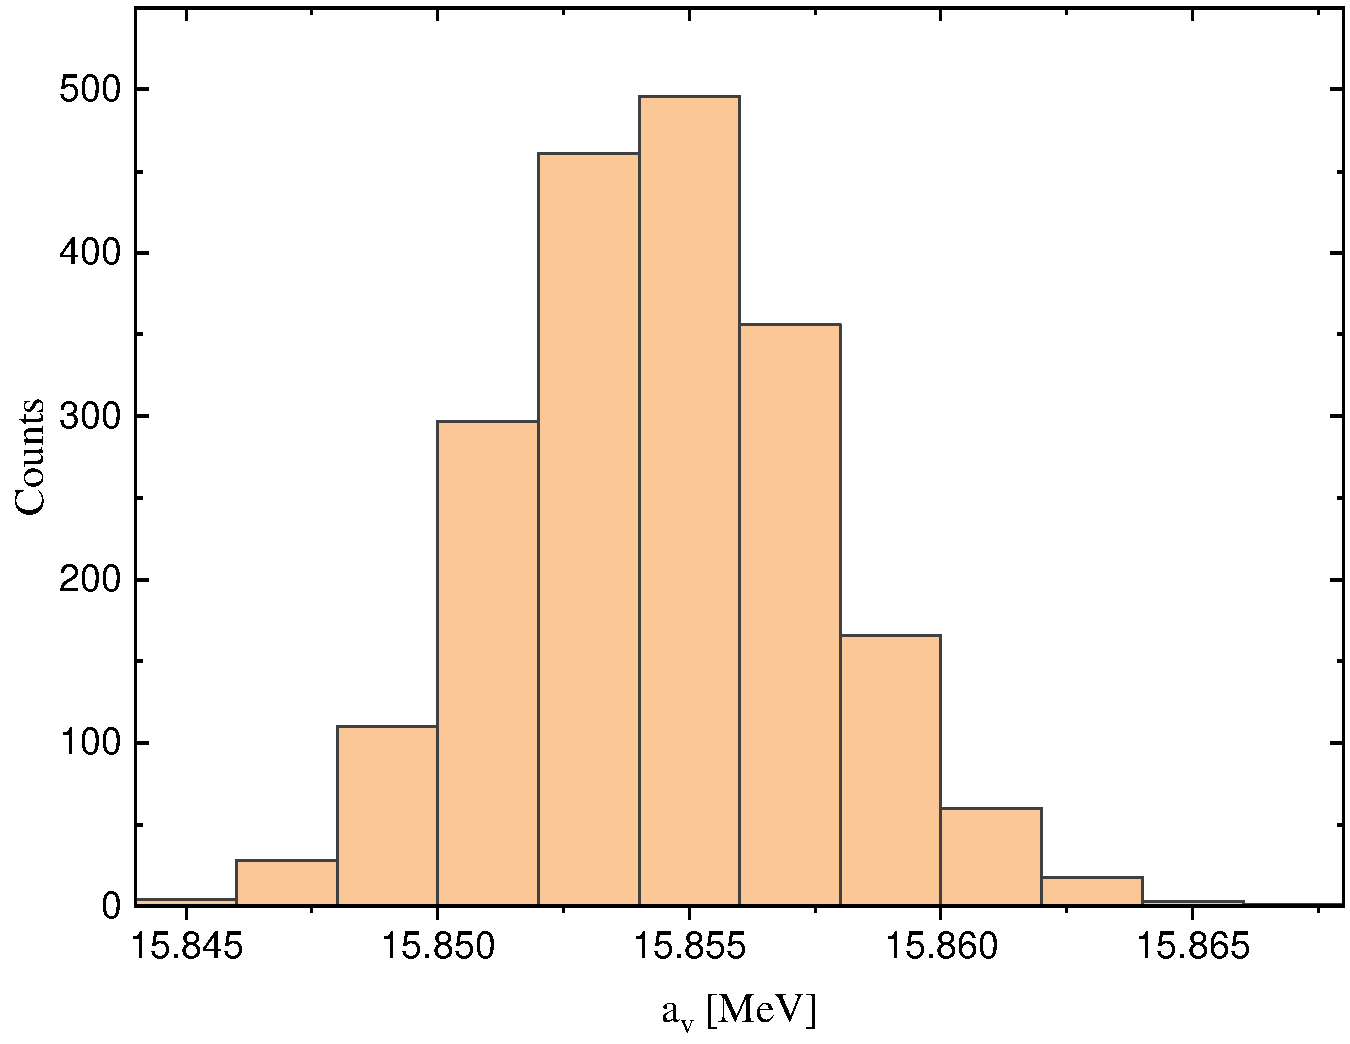
\includegraphics[width=0.6\textwidth]{UCBAME2003.pdf}
\caption{利用uncorrelated bootstrap(UCB)方法得到的$L(a_v)$的分布,其不确定度为0.00312 MeV.\label{fig_UCBAME2003}}
\end{figure}

\section{2019.09.05}
今天在还是在重复文献\cite{RN569},昨天重复uncorrelated bootstrap(UCB)方法的结果与文献中的结果不一致的原因还没有找到,今天重复了一点frequency-domain bootstrap (FDB)的结果,如图\ref{fig_FDBAME2003r},发现我们的结果与文献\cite{RN569}中的FIG. 2基本一致但是还是存在一定的差异,可能的原因应该是我们取的液滴模型的参数与文献\cite{RN569}中用的不一致。
\begin{figure}[H]
\centering
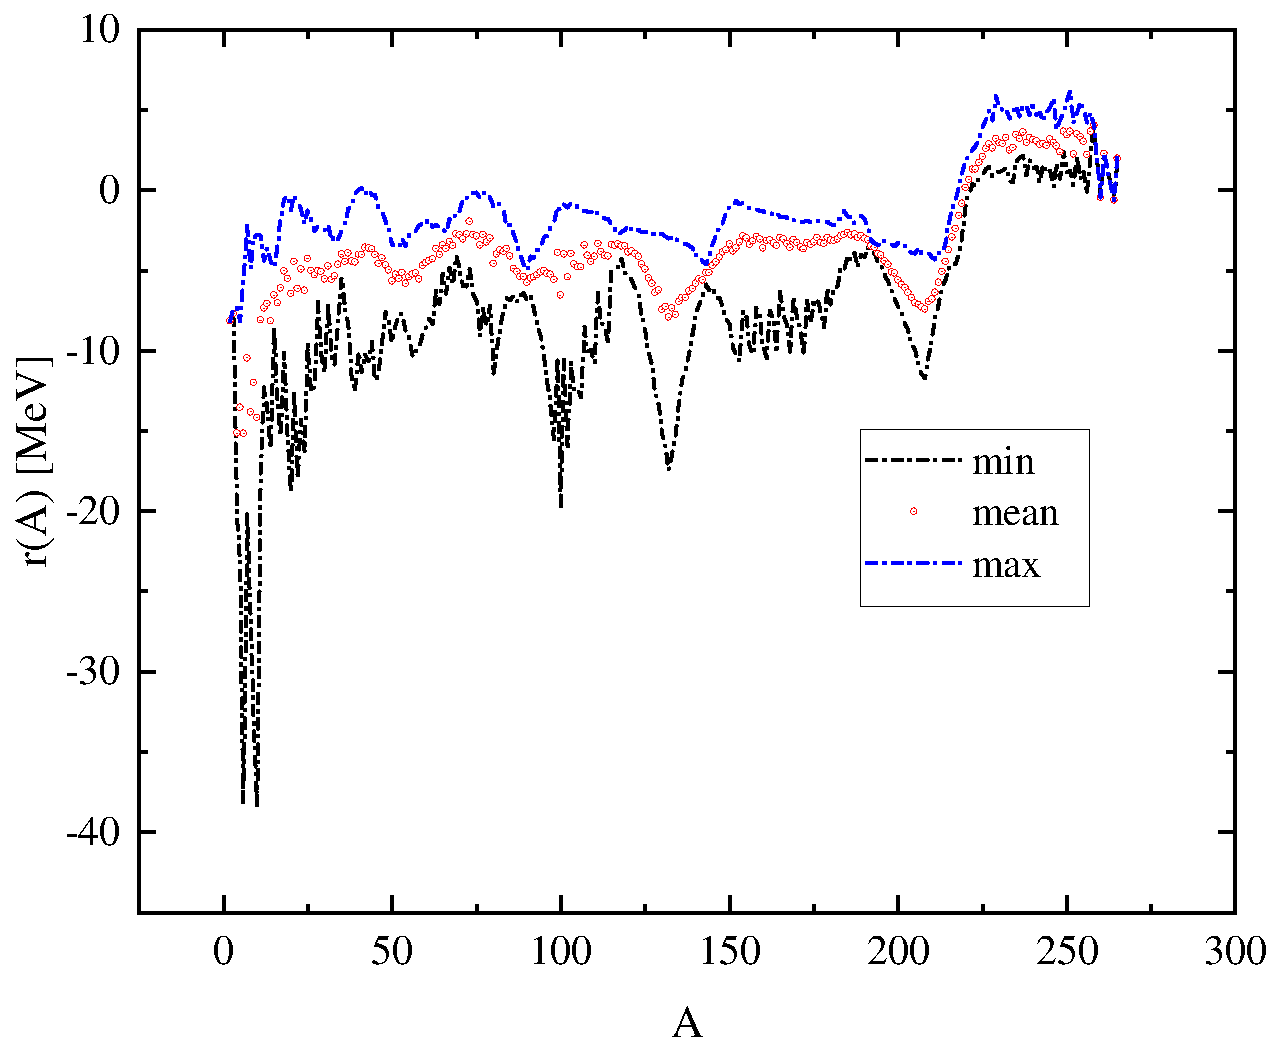
\includegraphics[width=0.6\textwidth]{FDBAME2003r.pdf}
\caption{液滴模型计算的结核能与AME2003质量表中给出的结合能的残差$r(A)$.\label{fig_FDBAME2003r}}
\end{figure}

\section{2019.09.06}
今天的主要工作是给出了重复了文献\cite{RN569}中的FIG. 3,重复的结果如图\ref{fig_FDBAME2003fig3}所示,两个结果基本一致但是还是存在一定的差异,可能的原因仍然应该是我们取的液滴模型的参数与文献\cite{RN569}中用的不一致。此外文献\cite{RN569}中对FDM方法的描述还有不太理解的地方。
\begin{figure}[H]
\centering
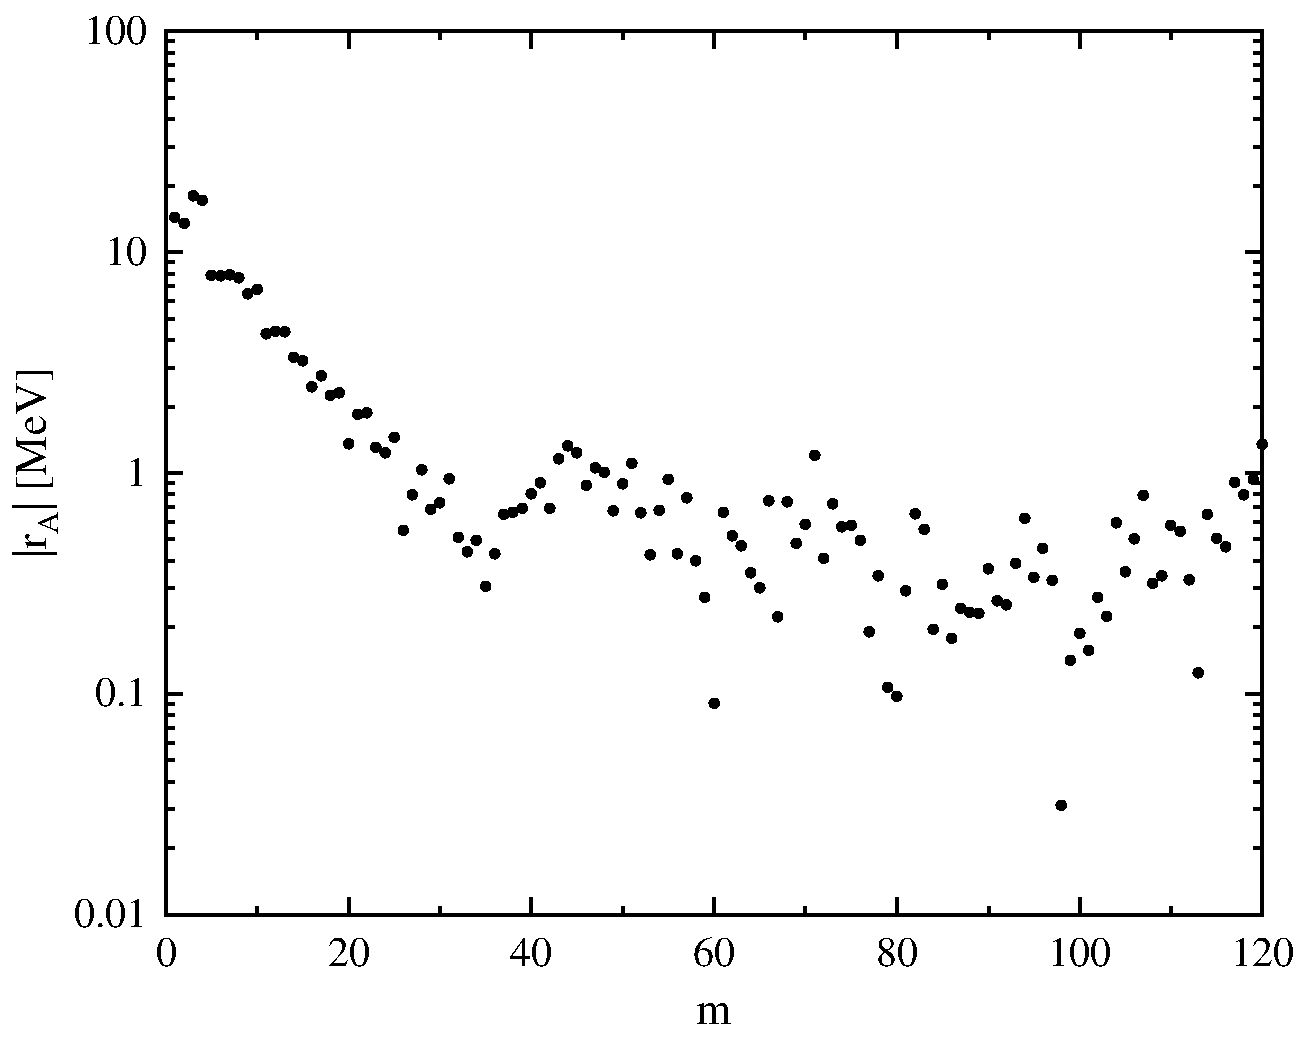
\includegraphics[width=0.6\textwidth]{FDBAME2003fig3.pdf}
\caption{液滴模型计算的结核能与AME2003质量表的残差$r(A)$通过傅里叶变换得到的结果.\label{fig_FDBAME2003fig3}}
\end{figure}

\section{2019.09.07}
今天的主要工作仍然是重复文献\cite{RN569}中结果,但是我们重复的文献\cite{RN569}中的FIG. 4的结果时,发现与我们得到的傅里叶反变换的结果(图\ref{fig_FDBAME2003fig4})存在极大的差异。
\begin{figure}[H]
\centering
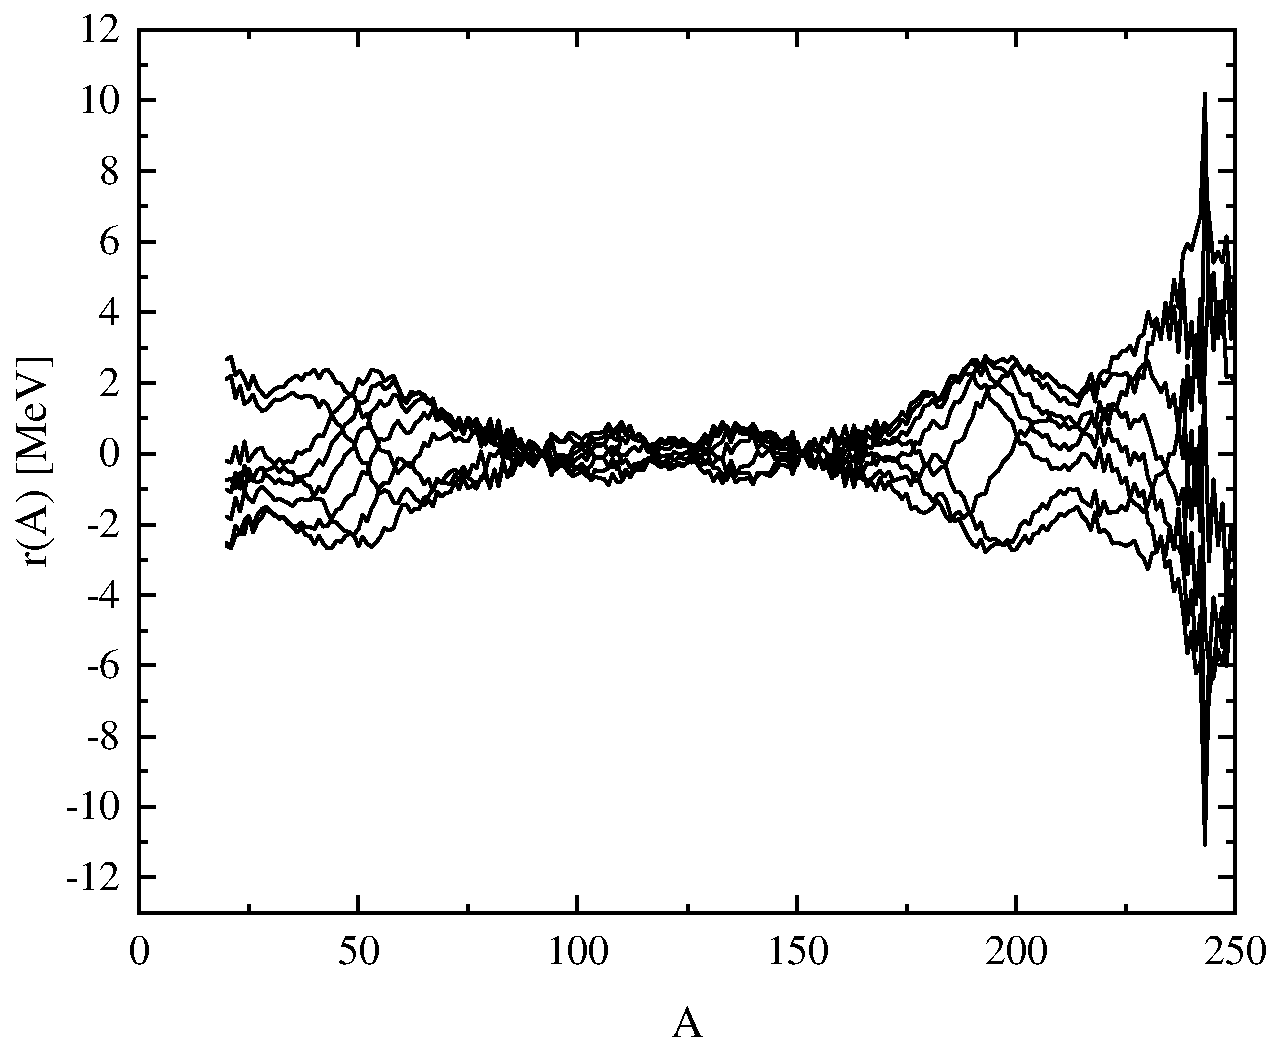
\includegraphics[width=0.6\textwidth]{FDBAME2003fig4.pdf}
\caption{重复的文献\cite{RN569}中的FIG. 4的傅里叶反变换得到的结果.\label{fig_FDBAME2003fig4}}
\end{figure}

\section{2019.09.09}
今天的主要工作是整理mass-date-based interaction部分的笔记,对这一部分的工作做一个截断。

\section{2019.09.10}
今天的主要工作仍然是整理mass-date-based interaction部分的笔记。

\section{2019.09.11}
今天的主要工作仍然是整理mass-date-based interaction部分的笔记。

\section{2019.09.16}
今天的主要工作仍然是整理mass-date-based interaction部分的笔记。

\section{2019.09.17}
今天的主要工作仍然是整理mass-date-based interaction部分的笔记,并且重新拟合并给出了新的图。

\section{2019.09.18}
今天的工作主要是为明天的行程做准备,以及重新对以前的计算结果进行了重新拟合。

\section{2019.09.19}
今天的工作主要是出发赶往郑州,参加2019年中国物理学会秋季会议。

\section{2019.09.20}
今天的工作主要参加2019年中国物理学会秋季会议,主要听了四个大会报告:《中国散裂中子源》陈和声、《Piezotronics and Piezo-phototronics of the Third Generation Semiconductors》王中林、《Laser ARPES on High Temperature Superconductors》周兴江、《超高品质因子微腔光学》肖云峰。
\begin{figure}[H]
\centering
\includegraphics[width=0.6\textwidth]{figure/CPS.jpg}
\caption{2019年中国物理学会(CPS)秋季会议开幕式.\label{fig_CPS}}
\end{figure}

\section{2019.09.21}
今天的工作主要参加2019年中国物理学会秋季会议的核物理与加速器物理分会场的报告,其中着重听了《原子核的手征对称性》赵鹏巍、《原子核的热激发形状相变》张炜两个报告,并copy了今天所有报告的PPT。
\begin{figure}[H]
\centering
\includegraphics[width=0.6\textwidth]{figure/CPS_B.jpg}
\caption{2019-CPS-核物理与加速器物理分会场.\label{fig_CPS_B}}
\end{figure}

\section{2019.09.22}
今天的工作主要参加2019年中国物理学会秋季会议的核物理与加速器物理分会场的报告,其中着重听了《原子核的对称性及其破缺》刘玉鑫、《伽马光核物理一些研究进展》罗文两个报告。
\begin{figure}[H]
\centering
\includegraphics[width=0.6\textwidth]{figure/CPS_B2.jpg}
\caption{2019-CPS-核物理与加速器物理分会场9.22.\label{fig_CPS_B2}}
\end{figure}

\section{2019.09.23}
今天从郑州出发回到学校。

\section{2019.09.24}
今天基本把拟合结果整理完了。

\section{2019.09.25}
今天把所有的拟合结果进行了汇总并进行了分析。

\section{2019.09.26}
今天寻找了原子核半径的实验数据,并利用这些数据计算了原子核的密度[${\rm keV/fm}^3$]分布:
\begin{figure}[H]
\centering
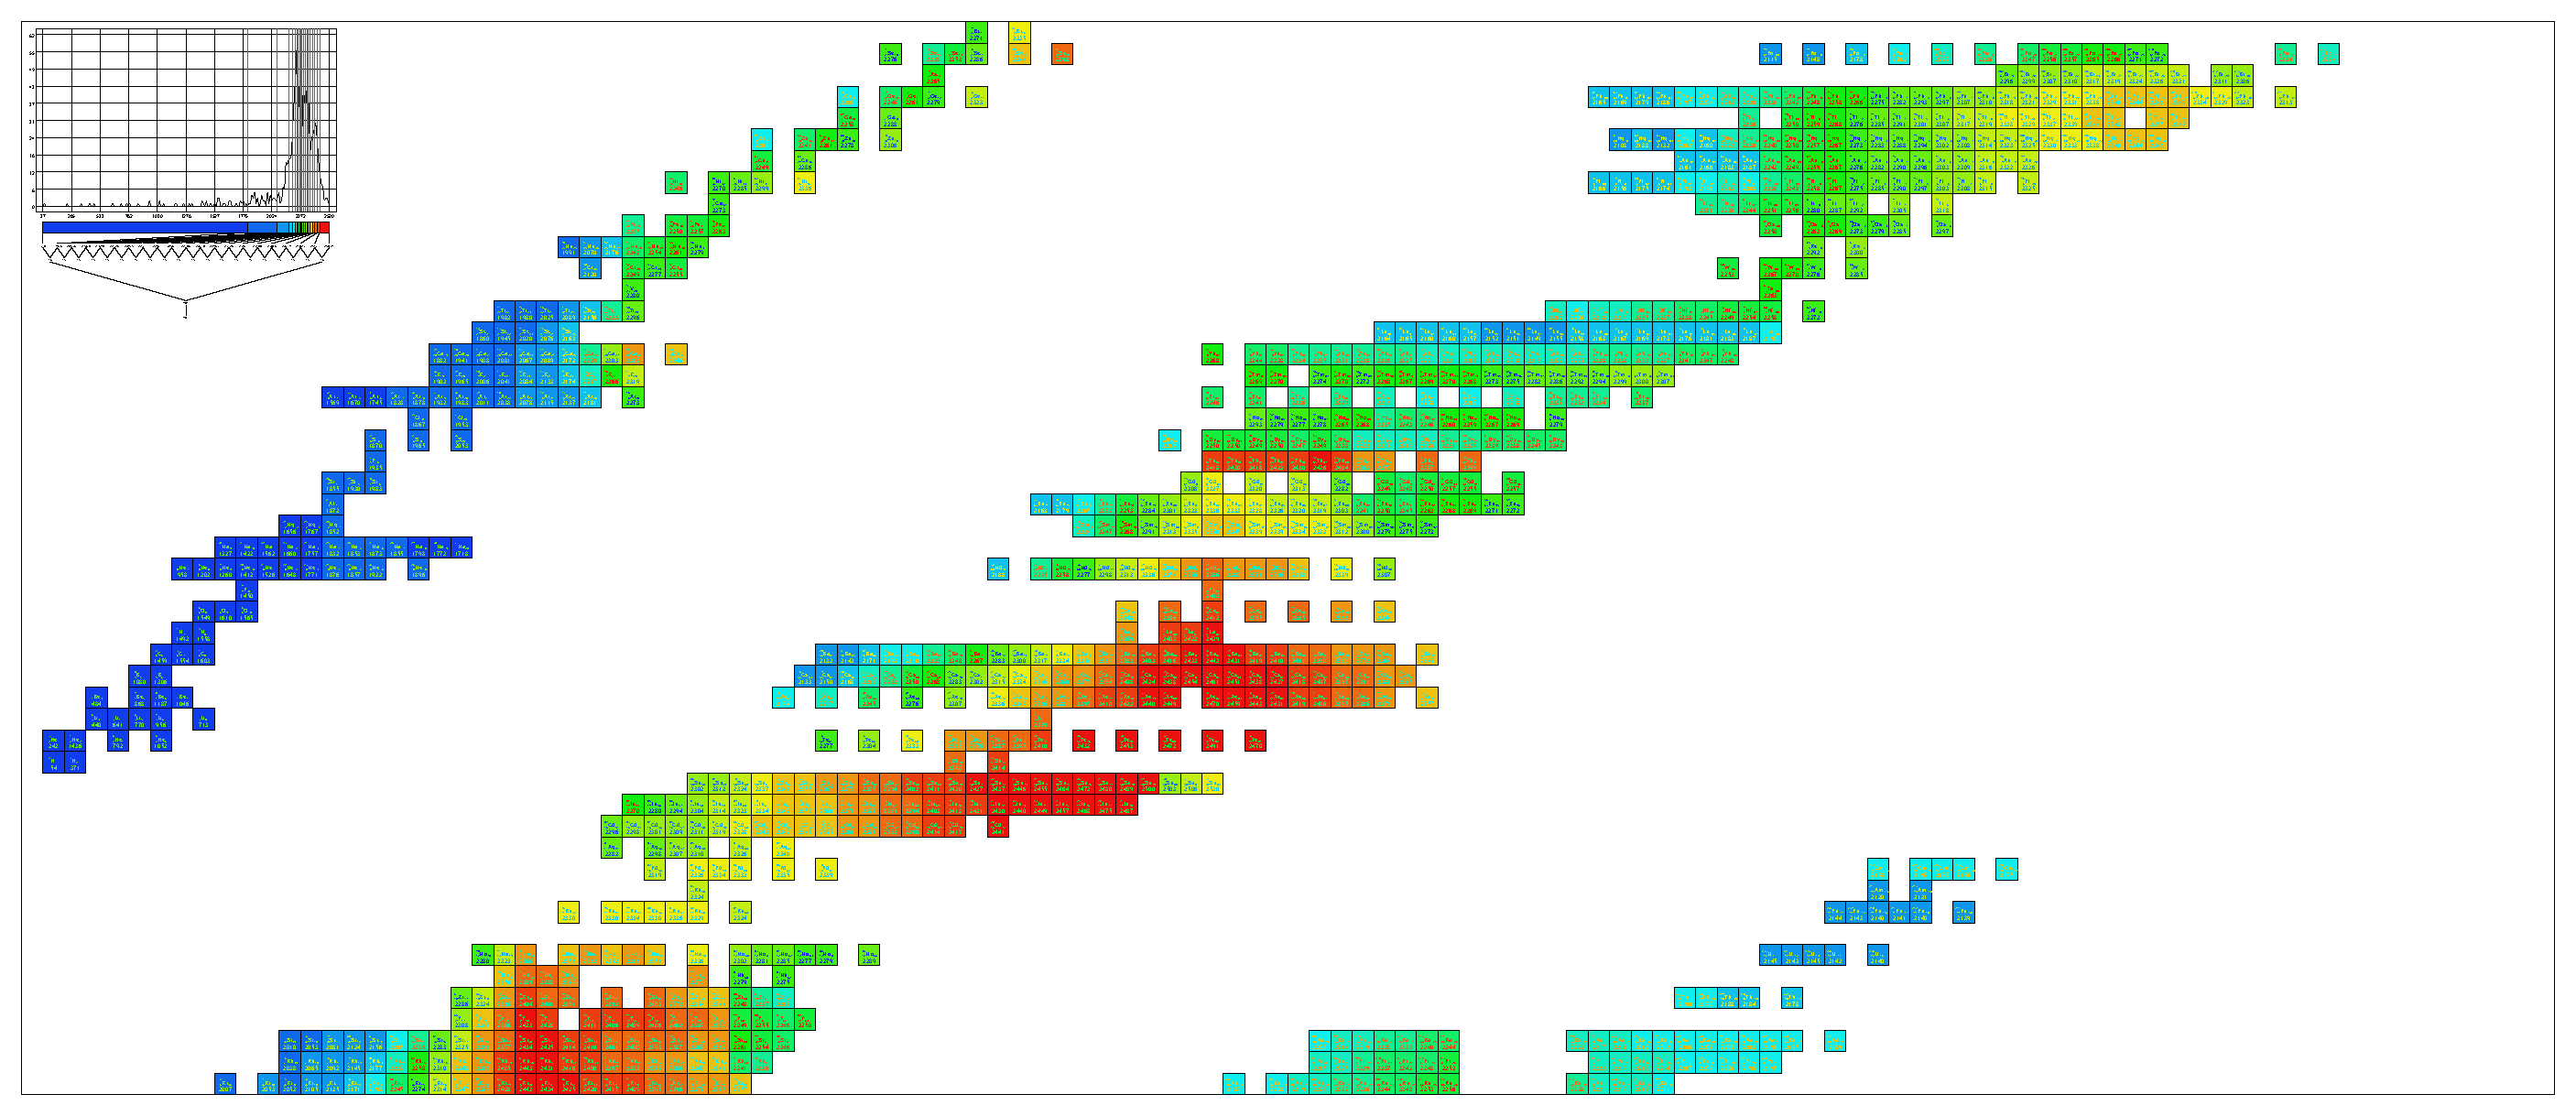
\includegraphics[width=0.6\textwidth]{figure/density.pdf}
\caption{原子核的密度[${\rm keV/fm}^3$]分布.\label{fig_density}}
\end{figure}

\section{2019.09.27}
今天的主要工作是总结参加的CPS2019秋季会议,并且准备周天用ppt讲一下。

\section{2019.09.28}
今天的主要工作是准备周天讲的ppt。

\section{2019.09.29}
今天的主要工作是将前面整理的质量相关的笔记整理为文章的格式。

\section{2019.09.30}
今天的主要工作是将前面整理的质量相关的笔记整理为文章的格式。

\section{2019.10.01}
今天的主要工作是将前面整理的质量相关的文章,此外还学习了一些分析力学的基础的知识。

\section{2019.10.02}
今天的主要工作是将前面整理的质量相关的文章,此外还学习了一些分析力学的基础的知识。

\section{2019.10.09}
今天的主要工作是阅读相关的文献将前面整理的质量相关的文章。

\section{2019.10.10}
今天的主要工作是阅读相关的文献将前面整理的质量相关的文章。